\documentclass[11pt]{article}

% =========================
% Packages
% =========================
\usepackage[margin=0.78in]{geometry}
\usepackage{amsmath,amssymb,amsfonts,mathtools}
\usepackage{booktabs,array,tabularx,longtable,multirow}
\usepackage{enumitem}
\usepackage[most]{tcolorbox}
\usepackage{xcolor}
\usepackage{fancyhdr}
\usepackage{titlesec}
\usepackage{hyperref}
\usepackage{lastpage}
\usepackage{setspace}
\usepackage{tikz}
\usepackage{pgfplots}
\usepackage{needspace}
\usepackage{caption}
\usepackage{multicol}
\usepackage{graphicx}
\usepackage{amsthm}
\usepackage{mathrsfs}
\usepackage{bm}
\usepackage{float}
\usetikzlibrary{calc,arrows.meta,positioning,decorations.pathreplacing,patterns}

\pgfplotsset{compat=1.18}
\setstretch{1.14}
\setlength{\parindent}{0pt}
\setlength{\parskip}{0.45em}
\setlist[itemize]{leftmargin=1.8em}
\setlist[enumerate]{leftmargin=2em}

% =========================
% Colors
% =========================
\definecolor{novelPurple}{RGB}{98,54,255}
\definecolor{novelPurpleDark}{RGB}{72,34,204}
\definecolor{novelPurpleLight}{RGB}{243,239,255}
\definecolor{novelPurpleLine}{RGB}{165,135,255}
\definecolor{npgray}{RGB}{78,78,78}
\definecolor{softgray}{RGB}{246,246,250}
\definecolor{softlav}{RGB}{249,247,255}
\definecolor{greencheck}{RGB}{24,128,88}
\definecolor{warmred}{RGB}{188,54,54}
\definecolor{nporange}{RGB}{223,121,36}
\definecolor{npgreen}{RGB}{67,142,103}
\definecolor{npred}{RGB}{180,54,54}

% =========================
% Hyperref
% =========================
\hypersetup{
    colorlinks=true,
    linkcolor=novelPurpleDark,
    urlcolor=novelPurpleDark,
    citecolor=novelPurpleDark
}

% =========================
% Header / Footer
% =========================
\pagestyle{fancy}
\fancyhf{}
\fancyhead[L]{\textbf{Novel Prep Learning Center}}
\fancyhead[R]{\textbf{AP Calculus AB/BC --- Unit 5}}
\fancyfoot[C]{\textcolor{novelPurpleDark}{\thepage\ /\ \pageref{LastPage}}}
\renewcommand{\headrulewidth}{0.4pt}
\renewcommand{\footrulewidth}{0pt}

% =========================
% Numbering / TOC
% =========================
\setcounter{secnumdepth}{3}
\setcounter{tocdepth}{3}

% =========================
% Section styles
% =========================
\titleformat{\section}
{\Large\bfseries\color{novelPurpleDark}}{\thesection.}{0.6em}{}

\titleformat{\subsection}
{\large\bfseries\color{novelPurple}}{\thesubsection.}{0.6em}{}

\titleformat{\subsubsection}
{\normalsize\bfseries\color{novelPurpleDark}}{\thesubsubsection.}{0.6em}{}

% =========================
% Boxes
% =========================
\tcbset{
  enhanced,
  sharp corners,
  boxrule=1pt
}

\newtcolorbox{theorybox}[1]{
  colback=white,
  colframe=novelPurple,
  colbacktitle=novelPurple,
  coltitle=white,
  title=\textbf{#1},
  fonttitle=\bfseries,
  sharp corners,
  breakable
}

\newtcolorbox{notebox}[1]{
  colback=novelPurpleLight,
  colframe=novelPurple,
  colbacktitle=novelPurple,
  coltitle=white,
  title=\textbf{#1},
  fonttitle=\bfseries,
  sharp corners,
  breakable
}

\newtcolorbox{skillbox}[1]{
  colback=softlav,
  colframe=novelPurpleDark,
  colbacktitle=novelPurpleDark,
  coltitle=white,
  title=\textbf{#1},
  fonttitle=\bfseries,
  sharp corners,
  breakable
}

\newtcolorbox{summarybox}[1]{
  colback=softgray,
  colframe=novelPurpleDark,
  colbacktitle=novelPurpleDark,
  coltitle=white,
  title=\textbf{#1},
  fonttitle=\bfseries,
  sharp corners,
  breakable
}

\newtcolorbox{practicebox}[1]{
  colback=white,
  colframe=novelPurpleLine,
  colbacktitle=novelPurpleLine,
  coltitle=black,
  title=\textbf{#1},
  fonttitle=\bfseries,
  sharp corners,
  breakable
}

\newtcolorbox{homeworkset}[1]{
  colback=white,
  colframe=novelPurpleDark,
  colbacktitle=novelPurpleDark,
  coltitle=white,
  title=\textbf{#1},
  fonttitle=\bfseries,
  sharp corners,
  breakable
}

\newcommand{\hwspace}{\vspace{0.8em}\hrule\vspace{0.8em}}

% =========================
% Commands
% =========================
\newcounter{examplectr}[subsection]
\renewcommand{\theexamplectr}{\thesubsection.\arabic{examplectr}}

\newcommand{\example}[1]{%
\refstepcounter{examplectr}
\Needspace{8\baselineskip}
\noindent{\color{novelPurpleDark}\textbf{Example \theexamplectr.}} \textbf{#1}\par
}

\newcommand{\solution}{\noindent{\textbf{Solution.}}}

\newcommand{\apcheckpoint}[1]{%
\begin{skillbox}{AP Checkpoint}
#1
\end{skillbox}
}

\newcommand{\unitchapter}[1]{%
\newpage
\subsection{#1}
}

\newcommand{\unitsubtopic}[1]{%
\subsubsection{#1}
}

% =========================
% Figures
% =========================
\newcommand{\unitcoverfigure}{
\begin{tikzpicture}[scale=1]
\fill[softlav,rounded corners=22pt] (-6.2,-1.8) rectangle (6.2,1.8);
\draw[novelPurple, line width=1.1pt, rounded corners=22pt] (-6.2,-1.8) rectangle (6.2,1.8);

% left: Rolle/MVT
\begin{scope}[shift={(-4.1,0)}]
\draw[novelPurpleDark, line width=0.9pt, ->] (-1.55,0)--(1.55,0);
\draw[novelPurpleDark, line width=0.9pt, ->] (0,-0.15)--(0,1.6);
\draw[novelPurple, line width=1.15pt, domain=-1.1:1.1, samples=120]
plot (\x,{1.1-0.7*\x*\x});
\draw[gray!50,dashed] (-1.0,0)--(-1.0,0.4);
\draw[gray!50,dashed] (1.0,0)--(1.0,0.4);
\draw[gray!50,dashed] (0,0)--(0,1.1);
\fill[npred] (-1.0,0.4) circle (1.4pt);
\fill[npred] (1.0,0.4) circle (1.4pt);
\fill[npred] (0,1.1) circle (1.4pt);
\node[text=npgray] at (0,-0.45) {\small Rolle / MVT};
\end{scope}

% middle: first derivative test
\begin{scope}[shift={(0,0)}]
\draw[novelPurpleDark, line width=0.9pt, ->] (-1.55,0)--(1.55,0);
\draw[novelPurpleDark, line width=0.9pt, ->] (0,-0.25)--(0,1.7);
\draw[novelPurple, line width=1.15pt, smooth, domain=-1.1:1.1, samples=160]
plot (\x,{0.3*\x*\x*\x-0.5*\x+0.7});
\node[text=npgray] at (-0.7,1.35) {\small $(-)$};
\node[text=npgray] at (0.7,1.35) {\small $(+)$};
\node[text=npgray] at (0,-0.45) {\small derivative tests};
\end{scope}

% right: optimization
\begin{scope}[shift={(4.0,0)}]
\draw[novelPurpleDark, line width=0.9pt, ->] (-1.55,0)--(1.55,0);
\draw[novelPurpleDark, line width=0.9pt, ->] (0,-0.15)--(0,1.8);
\draw[novelPurple, line width=1.15pt, smooth, domain=-1.1:1.1, samples=160]
plot (\x,{1.25-0.65*(\x)^2});
\draw[nporange, line width=0.95pt] (-0.65,0)--(-0.65,0.98)--(0.65,0.98)--(0.65,0);
\node[text=npgray] at (0,-0.45) {\small optimization};
\end{scope}

\node[align=center] at (0,-2.35) ;
\end{tikzpicture}
}

\newcommand{\rollefigure}{
\begin{center}
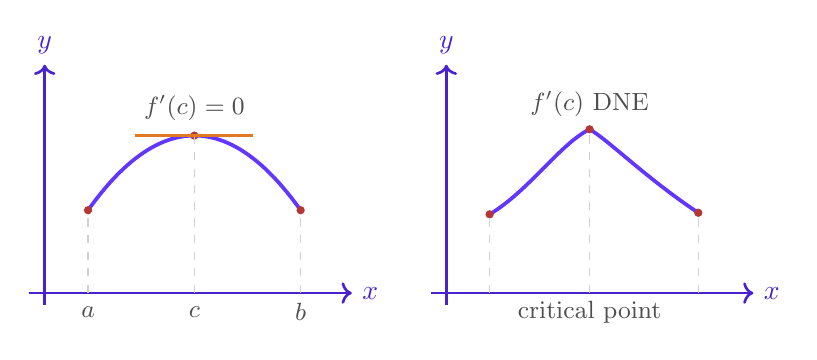
\begin{tikzpicture}[x=1cm,y=1cm]

    % Left panel
    \begin{scope}[shift={(0,0)}]
        \draw[novelPurpleDark, line width=0.95pt, ->] (-0.2,0) -- (3.9,0) node[right] {$x$};
        \draw[novelPurpleDark, line width=0.95pt, ->] (0,-0.15) -- (0,2.9) node[above] {$y$};
        \draw[novelPurple, line width=1.35pt, smooth, samples=160, domain=0.55:3.25]
            plot (\x,{2.0 - 0.52*(\x-1.9)^2});
        \pgfmathsetmacro{\ya}{2.0 - 0.52*(0.55-1.9)^2}
        \pgfmathsetmacro{\yb}{2.0 - 0.52*(3.25-1.9)^2}
        \fill[npred] (0.55,\ya) circle (1.5pt);
        \fill[npred] (1.9,2.0) circle (1.5pt);
        \fill[npred] (3.25,\yb) circle (1.5pt);
        \draw[gray!35, dashed] (0.55,0) -- (0.55,\ya);
        \draw[gray!35, dashed] (1.9,0) -- (1.9,2.0);
        \draw[gray!35, dashed] (3.25,0) -- (3.25,\yb);
        \draw[nporange, line width=1.05pt] (1.15,2.0) -- (2.65,2.0);
        \node[text=npgray] at (1.9,2.35) {\small $f'(c)=0$};
        \node[text=npgray] at (0.55,-0.24) {\small $a$};
        \node[text=npgray] at (1.9,-0.24) {\small $c$};
        \node[text=npgray] at (3.25,-0.24) {\small $b$};
    \end{scope}

    % Right panel
    \begin{scope}[shift={(5.1,0)}]
        \draw[novelPurpleDark, line width=0.95pt, ->] (-0.2,0) -- (3.9,0) node[right] {$x$};
        \draw[novelPurpleDark, line width=0.95pt, ->] (0,-0.15) -- (0,2.9) node[above] {$y$};
        \draw[novelPurple, line width=1.35pt]
            (0.55,1.0)
            .. controls (1.05,1.3) and (1.45,1.9) .. (1.82,2.08);
        \draw[novelPurple, line width=1.35pt]
            (1.82,2.08)
            .. controls (2.05,1.95) and (2.55,1.45) .. (3.2,1.02);
        \fill[npred] (0.55,1.0) circle (1.5pt);
        \fill[npred] (1.82,2.08) circle (1.5pt);
        \fill[npred] (3.2,1.02) circle (1.5pt);
        \draw[gray!35, dashed] (0.55,0) -- (0.55,1.0);
        \draw[gray!35, dashed] (1.82,0) -- (1.82,2.08);
        \draw[gray!35, dashed] (3.2,0) -- (3.2,1.02);
        \node[text=npgray] at (1.82,2.4) {\small $f'(c)$ DNE};
        \node[text=npgray] at (1.82,-0.24) {\small critical point};
    \end{scope}

\end{tikzpicture}
\end{center}
}

\newcommand{\mvttangentfigure}{
\begin{center}
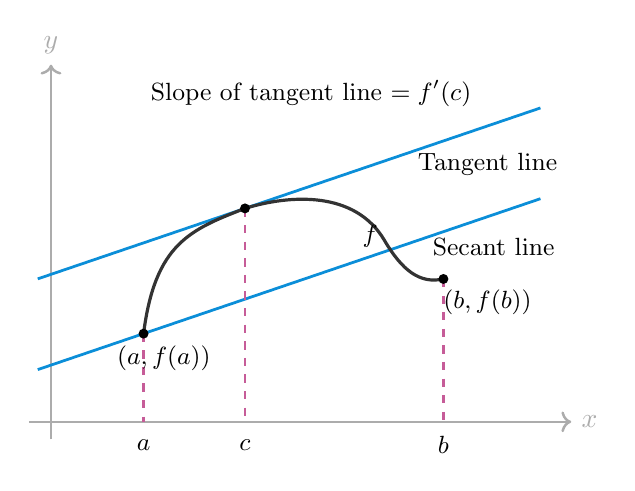
\begin{tikzpicture}[x=1.12cm,y=1.12cm]
    \coordinate (A) at (1.05,1.00);
    \coordinate (C) at (2.20,2.42);
    \coordinate (B) at (4.45,1.62);
    \pgfmathsetmacro{\m}{0.34}

    \draw[gray!65, line width=0.9pt, ->] (-0.25,0) -- (5.9,0) node[right] {$x$};
    \draw[gray!65, line width=0.9pt, ->] (0,-0.2) -- (0,4.05) node[above] {$y$};

    \draw[cyan!75!blue, line width=1.0pt]
        (-0.15,{1.00+\m*(-0.15-1.05)}) -- (5.55,{1.00+\m*(5.55-1.05)});

    \draw[cyan!75!blue, line width=1.0pt]
        (-0.15,{2.42+\m*(-0.15-2.20)}) -- (5.55,{2.42+\m*(5.55-2.20)});

    \draw[black!80, line width=1.15pt]
        (A)
        .. controls (1.18,2.02) and (1.58,2.18) .. (C)
        .. controls (2.72,2.58) and (3.45,2.62) .. (3.78,2.06)
        .. controls (3.98,1.72) and (4.18,1.56) .. (B);

    \draw[magenta!55!gray, dashed, line width=0.9pt] (A) -- (1.05,0);
    \draw[magenta!55!gray, dashed, line width=0.9pt] (C) -- (2.20,0);
    \draw[magenta!55!gray, dashed, line width=0.9pt] (B) -- (4.45,0);

    \fill[black] (A) circle (1.8pt);
    \fill[black] (C) circle (1.8pt);
    \fill[black] (B) circle (1.8pt);

    \node[font=\small] at (2.95,3.72) {Slope of tangent line $= f'(c)$};
    \node[font=\small] at (4.95,2.92) {Tangent line};
    \node[font=\small] at (5.02,1.98) {Secant line};
    \node[font=\small] at (3.62,2.10) {$f$};
    \node[font=\small] at (1.28,0.72) {$(a,f(a))$};
    \node[font=\small] at (4.95,1.36) {$(b,f(b))$};
    \node[font=\small] at (1.05,-0.26) {$a$};
    \node[font=\small] at (2.20,-0.26) {$c$};
    \node[font=\small] at (4.45,-0.26) {$b$};
\end{tikzpicture}
\end{center}
}

\newcommand{\extremaoverviewfigure}{
\begin{center}
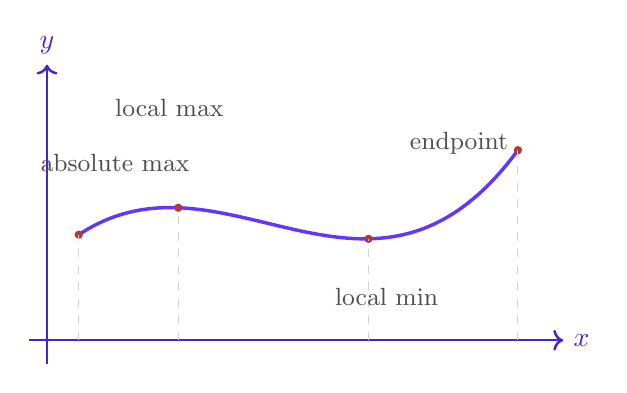
\begin{tikzpicture}[x=1.15cm,y=1.0cm]
    \draw[novelPurpleDark, line width=0.9pt, ->] (-0.2,0) -- (5.7,0) node[right] {$x$};
    \draw[novelPurpleDark, line width=0.9pt, ->] (0,-0.3) -- (0,3.5) node[above] {$y$};
    \draw[novelPurple, line width=1.25pt, smooth, samples=220, domain=0.35:5.2]
        plot (\x,{0.08*(\x-0.7)*(\x-2.2)*(\x-4.4)+1.55});
    \fill[npred] (0.35,{0.08*(0.35-0.7)*(0.35-2.2)*(0.35-4.4)+1.55}) circle (1.5pt);
    \fill[npred] (1.45,{0.08*(1.45-0.7)*(1.45-2.2)*(1.45-4.4)+1.55}) circle (1.5pt);
    \fill[npred] (3.55,{0.08*(3.55-0.7)*(3.55-2.2)*(3.55-4.4)+1.55}) circle (1.5pt);
    \fill[npred] (5.2,{0.08*(5.2-0.7)*(5.2-2.2)*(5.2-4.4)+1.55}) circle (1.5pt);
    \draw[gray!35,dashed] (0.35,0)--(0.35,{0.08*(0.35-0.7)*(0.35-2.2)*(0.35-4.4)+1.55});
    \draw[gray!35,dashed] (1.45,0)--(1.45,{0.08*(1.45-0.7)*(1.45-2.2)*(1.45-4.4)+1.55});
    \draw[gray!35,dashed] (3.55,0)--(3.55,{0.08*(3.55-0.7)*(3.55-2.2)*(3.55-4.4)+1.55});
    \draw[gray!35,dashed] (5.2,0)--(5.2,{0.08*(5.2-0.7)*(5.2-2.2)*(5.2-4.4)+1.55});
    \node[text=npgray] at (1.35,2.95) {\small local max};
    \node[text=npgray] at (3.75,0.55) {\small local min};
    \node[text=npgray] at (0.75,2.25) {\small absolute max};
    \node[text=npgray] at (4.55,2.5) {\small endpoint};
\end{tikzpicture}
\end{center}
}

\newcommand{\localvsabsolutefigure}{
\begin{center}
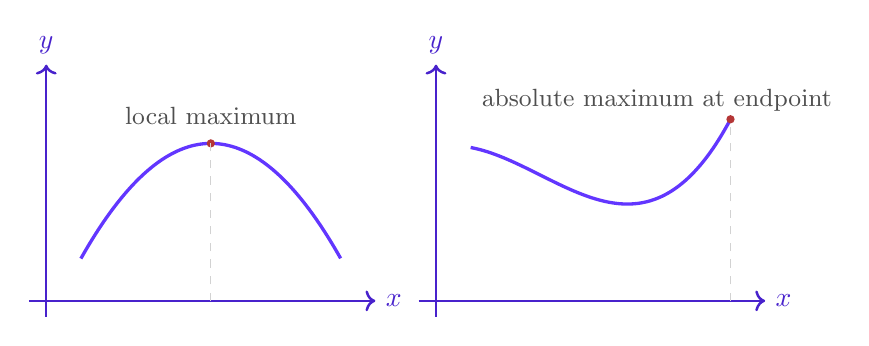
\begin{tikzpicture}[x=1.1cm,y=1.0cm]
    \begin{scope}[shift={(0,0)}]
        \draw[novelPurpleDark, line width=0.9pt, ->] (-0.2,0) -- (3.8,0) node[right] {$x$};
        \draw[novelPurpleDark, line width=0.9pt, ->] (0,-0.2) -- (0,3.0) node[above] {$y$};
        \draw[novelPurple, line width=1.2pt, smooth, samples=160, domain=0.4:3.4]
            plot (\x,{2.0-0.65*(\x-1.9)^2});
        \fill[npred] (1.9,2.0) circle (1.5pt);
        \draw[gray!35,dashed] (1.9,0)--(1.9,2.0);
        \node[text=npgray] at (1.9,2.35) {\small local maximum};
    \end{scope}
    \begin{scope}[shift={(4.5,0)}]
        \draw[novelPurpleDark, line width=0.9pt, ->] (-0.2,0) -- (3.8,0) node[right] {$x$};
        \draw[novelPurpleDark, line width=0.9pt, ->] (0,-0.2) -- (0,3.0) node[above] {$y$};
        \draw[novelPurple, line width=1.2pt, smooth, samples=180, domain=0.4:3.4]
            plot (\x,{0.18*(\x-1.2)^3-0.55*(\x-1.2)+1.6});
        \fill[npred] (3.4,{0.18*(3.4-1.2)^3-0.55*(3.4-1.2)+1.6}) circle (1.5pt);
        \draw[gray!35,dashed] (3.4,0)--(3.4,{0.18*(3.4-1.2)^3-0.55*(3.4-1.2)+1.6});
        \node[text=npgray] at (2.55,2.55) {\small absolute maximum at endpoint};
    \end{scope}
\end{tikzpicture}
\end{center}
}

\newcommand{\criticalfigure}{
\begin{center}
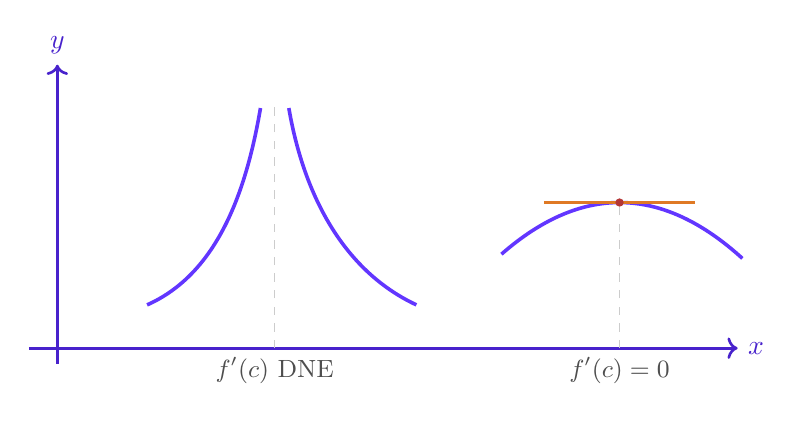
\begin{tikzpicture}[x=1.2cm,y=1.0cm]
    \draw[novelPurpleDark, line width=0.95pt, ->] (-0.3,0) -- (7.2,0) node[right] {$x$};
    \draw[novelPurpleDark, line width=0.95pt, ->] (0,-0.2) -- (0,3.6) node[above] {$y$};

    \begin{scope}[shift={(0.55,0)}]
        \draw[novelPurple, line width=1.3pt]
            (0.4,0.55) .. controls (1.15,0.95) and (1.45,2.0) .. (1.6,3.05);
        \draw[novelPurple, line width=1.3pt]
            (1.9,3.05) .. controls (2.05,2.0) and (2.45,1.0) .. (3.25,0.55);
        \draw[gray!40, dashed] (1.75,0) -- (1.75,3.1);
        \node[text=npgray] at (1.75,-0.28) {\small $f'(c)$ DNE};
    \end{scope}

    \begin{scope}[shift={(4.25,0)}]
        \draw[novelPurple, line width=1.3pt, smooth, samples=160, domain=0.45:3.0]
            plot (\x,{1.85-0.42*(\x-1.7)^2});
        \draw[nporange, line width=1.05pt] (0.9,1.85) -- (2.5,1.85);
        \draw[gray!40, dashed] (1.7,0) -- (1.7,1.85);
        \fill[npred] (1.7,1.85) circle (1.5pt);
        \node[text=npgray] at (1.7,-0.28) {\small $f'(c)=0$};
    \end{scope}
\end{tikzpicture}
\end{center}
}

\newcommand{\closedintervalextremafigure}{
\begin{center}
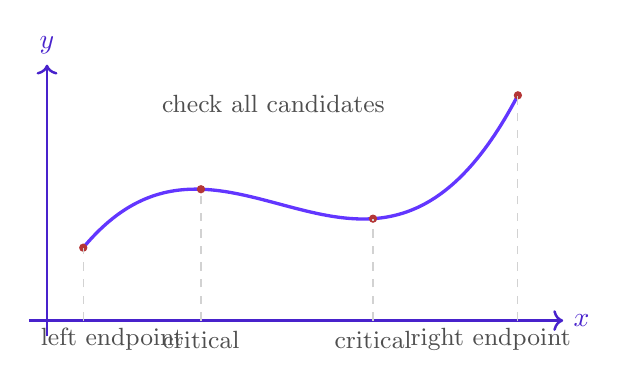
\begin{tikzpicture}[x=1.15cm,y=1.0cm]
    \draw[novelPurpleDark, line width=0.9pt, ->] (-0.2,0) -- (5.7,0) node[right] {$x$};
    \draw[novelPurpleDark, line width=0.9pt, ->] (0,-0.2) -- (0,3.25) node[above] {$y$};
    \draw[novelPurple, line width=1.2pt, smooth, samples=220, domain=0.4:5.2]
        plot (\x,{0.12*(\x-1.0)*(\x-2.5)*(\x-4.2)+1.5});
    \fill[npred] (0.4,{0.12*(0.4-1.0)*(0.4-2.5)*(0.4-4.2)+1.5}) circle (1.5pt);
    \fill[npred] (1.7,{0.12*(1.7-1.0)*(1.7-2.5)*(1.7-4.2)+1.5}) circle (1.5pt);
    \fill[npred] (3.6,{0.12*(3.6-1.0)*(3.6-2.5)*(3.6-4.2)+1.5}) circle (1.5pt);
    \fill[npred] (5.2,{0.12*(5.2-1.0)*(5.2-2.5)*(5.2-4.2)+1.5}) circle (1.5pt);
    \draw[gray!35,dashed] (0.4,0)--(0.4,{0.12*(0.4-1.0)*(0.4-2.5)*(0.4-4.2)+1.5});
    \draw[gray!35,dashed] (1.7,0)--(1.7,{0.12*(1.7-1.0)*(1.7-2.5)*(1.7-4.2)+1.5});
    \draw[gray!35,dashed] (3.6,0)--(3.6,{0.12*(3.6-1.0)*(3.6-2.5)*(3.6-4.2)+1.5});
    \draw[gray!35,dashed] (5.2,0)--(5.2,{0.12*(5.2-1.0)*(5.2-2.5)*(5.2-4.2)+1.5});
    \node[text=npgray] at (0.72,-0.24) {\small left endpoint};
    \node[text=npgray] at (1.7,-0.24) {\small critical};
    \node[text=npgray] at (3.6,-0.24) {\small critical};
    \node[text=npgray] at (4.9,-0.24) {\small right endpoint};
    \node[text=npgray] at (2.5,2.75) {\small check all candidates};
\end{tikzpicture}
\end{center}
}

\newcommand{\incdecfigure}{
\begin{center}
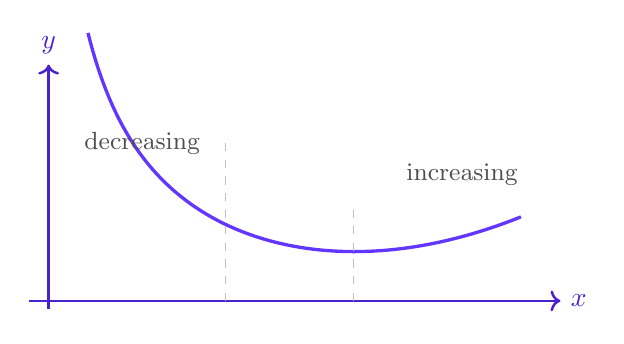
\begin{tikzpicture}[x=1.25cm,y=1.0cm]
\draw[novelPurpleDark, line width=0.9pt, ->] (-0.2,0)--(5.2,0) node[right] {$x$};
\draw[novelPurpleDark, line width=0.9pt, ->] (0,-0.1)--(0,3.0) node[above] {$y$};
\draw[novelPurple, line width=1.2pt, smooth, domain=0.4:4.8, samples=160]
plot (\x,{1.9/(\x+0.25)+0.12*(\x-2.4)^2});
\draw[gray!50,dashed] (1.8,0)--(1.8,2.0);
\draw[gray!50,dashed] (3.1,0)--(3.1,1.15);
\node[text=npgray] at (0.95,2.0) {\small decreasing};
\node[text=npgray] at (4.2,1.6) {\small increasing};
\end{tikzpicture}
\end{center}
}

\newcommand{\graphroadmapfigure}{
\begin{center}
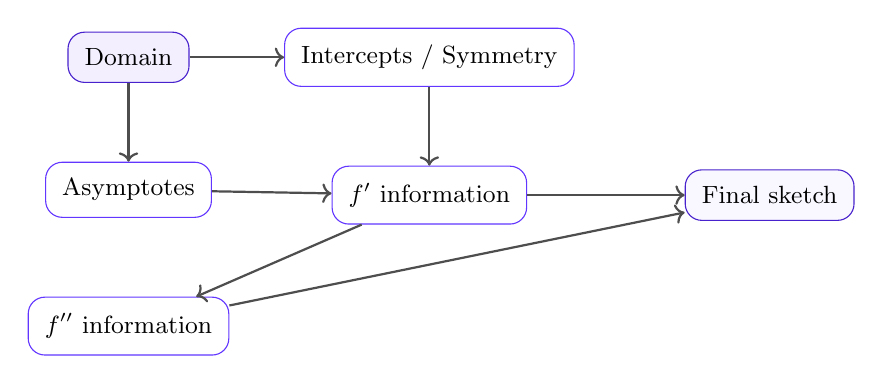
\begin{tikzpicture}[node distance=1.0cm and 1.2cm, every node/.style={font=\small}]
    \node[draw=novelPurpleDark, rounded corners=6pt, fill=novelPurpleLight, inner sep=6pt] (domain) {Domain};
    \node[draw=novelPurple, rounded corners=6pt, fill=white, inner sep=6pt, right=of domain] (intercepts) {Intercepts / Symmetry};
    \node[draw=novelPurple, rounded corners=6pt, fill=white, inner sep=6pt, below=of domain] (asym) {Asymptotes};
    \node[draw=novelPurple, rounded corners=6pt, fill=white, inner sep=6pt, below=of intercepts] (fp) {$f'$ information};
    \node[draw=novelPurple, rounded corners=6pt, fill=white, inner sep=6pt, below=of asym] (fpp) {$f''$ information};
    \node[draw=novelPurpleDark, rounded corners=6pt, fill=softlav, inner sep=6pt, right=2.0cm of fp] (final) {Final sketch};

    \draw[->, line width=0.8pt, color=npgray] (domain)--(intercepts);
    \draw[->, line width=0.8pt, color=npgray] (domain)--(asym);
    \draw[->, line width=0.8pt, color=npgray] (intercepts)--(fp);
    \draw[->, line width=0.8pt, color=npgray] (asym)--(fp);
    \draw[->, line width=0.8pt, color=npgray] (fp)--(fpp);
    \draw[->, line width=0.8pt, color=npgray] (fp)--(final);
    \draw[->, line width=0.8pt, color=npgray] (fpp)--(final);
\end{tikzpicture}
\end{center}
}

\newcommand{\rationalsketchfigure}{
\begin{center}
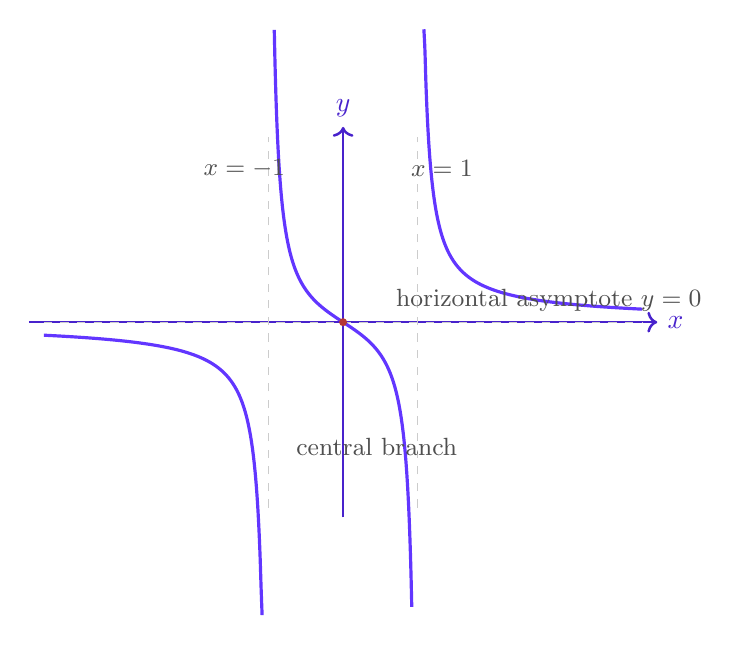
\begin{tikzpicture}[x=0.95cm,y=0.62cm]
    % axes
    \draw[novelPurpleDark, line width=0.9pt, ->] (-4.2,0)--(4.2,0) node[right] {$x$};
    \draw[novelPurpleDark, line width=0.9pt, ->] (0,-4.0)--(0,4.0) node[above] {$y$};

    % asymptotes
    \draw[gray!40,dashed] (-1,-3.8)--(-1,3.8);
    \draw[gray!40,dashed] (1,-3.8)--(1,3.8);
    \draw[gray!40,dashed] (-4.0,0)--(4.0,0);

    % clipped graph of y = x/(x^2-1)
    \draw[novelPurple, line width=1.15pt, smooth, samples=220, domain=-4:-1.08]
        plot (\x,{max(min((\x)/((\x)^2-1),6),-6)});
    \draw[novelPurple, line width=1.15pt, smooth, samples=220, domain=-0.92:0.92]
        plot (\x,{max(min((\x)/((\x)^2-1),6),-6)});
    \draw[novelPurple, line width=1.15pt, smooth, samples=220, domain=1.08:4]
        plot (\x,{max(min((\x)/((\x)^2-1),6),-6)});

    % key point
    \fill[npred] (0,0) circle (1.45pt);

    % labels
    \node[text=npgray] at (-1.32,3.15) {\small $x=-1$};
    \node[text=npgray] at (1.32,3.15) {\small $x=1$};
    \node[text=npgray] at (2.75,0.45) {\small horizontal asymptote $y=0$};
    \node[text=npgray] at (0.45,-2.55) {\small central branch};
\end{tikzpicture}
\end{center}
}

\newcommand{\firstderivfigure}{
\begin{center}
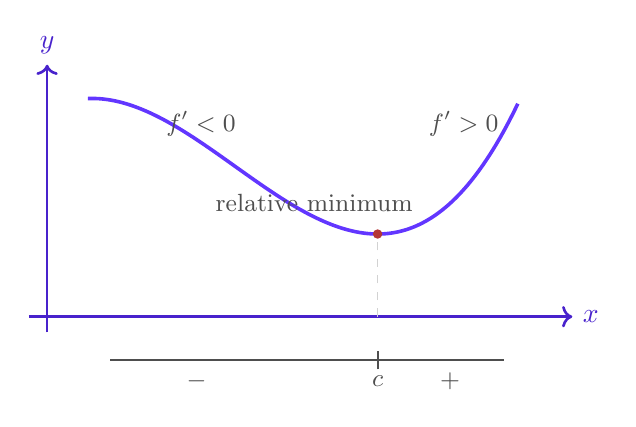
\begin{tikzpicture}[x=1.15cm,y=1.0cm]

    % axes
    \draw[novelPurpleDark, line width=0.95pt, ->] (-0.2,0) -- (5.8,0) node[right] {$x$};
    \draw[novelPurpleDark, line width=0.95pt, ->] (0,-0.2) -- (0,3.2) node[above] {$y$};

    % function with a clear relative minimum at c
    \draw[novelPurple, line width=1.3pt, smooth, samples=220, domain=0.45:5.2]
        plot (\x,{0.11*(\x-3.65)^3 + 0.52*(\x-3.65)^2 + 1.05});

    % minimum point c
    \pgfmathsetmacro{\xc}{3.65}
    \pgfmathsetmacro{\yc}{1.05}
    \fill[npred] (\xc,\yc) circle (1.7pt);

    % vertical guide
    \draw[gray!35,dashed] (\xc,0) -- (\xc,\yc);

    % labels on graph
    \node[text=npgray] at (1.7,2.45) {\small $f'<0$};
    \node[text=npgray] at (4.6,2.45) {\small $f'>0$};
    \node[text=npgray] at (2.95,1.45) {\small relative minimum};

    % sign chart under x-axis
    \draw[npgray, line width=0.8pt] (0.7,-0.55) -- (5.05,-0.55);
    \draw[npgray, line width=0.8pt] (\xc,-0.67) -- (\xc,-0.43);

    \node[text=npgray] at (1.65,-0.82) {\small $-$};
    \node[text=npgray] at (\xc,-0.82) {\small $c$};
    \node[text=npgray] at (4.45,-0.82) {\small $+$};

\end{tikzpicture}
\end{center}
}

\newcommand{\concavityfigure}{
\begin{center}
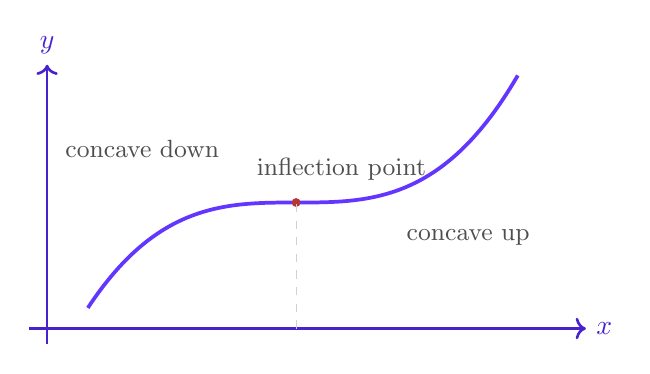
\begin{tikzpicture}[x=1.15cm,y=1.0cm]

    % axes
    \draw[novelPurpleDark, line width=0.95pt, ->] (-0.2,0) -- (5.95,0) node[right] {$x$};
    \draw[novelPurpleDark, line width=0.95pt, ->] (0,-0.2) -- (0,3.35) node[above] {$y$};

    % curve with stronger change in concavity
    \draw[novelPurple, line width=1.35pt, smooth, samples=240, domain=0.45:5.2]
        plot (\x,{0.11*(\x-2.75)^3 + 1.6});

    % inflection point
    \pgfmathsetmacro{\xc}{2.75}
    \pgfmathsetmacro{\yc}{1.6}
    \fill[npred] (\xc,\yc) circle (1.6pt);

    % vertical guide
    \draw[gray!35,dashed] (\xc,0) -- (\xc,\yc);

    % labels spread out
    \node[text=npgray] at (1.05,2.28) {\small concave down};
    \node[text=npgray] at (3.25,2.02) {\small inflection point};
    \node[text=npgray] at (4.65,1.15) {\small concave up};

\end{tikzpicture}
\end{center}
}

\newcommand{\fprimefdoublefigure}{
\begin{center}
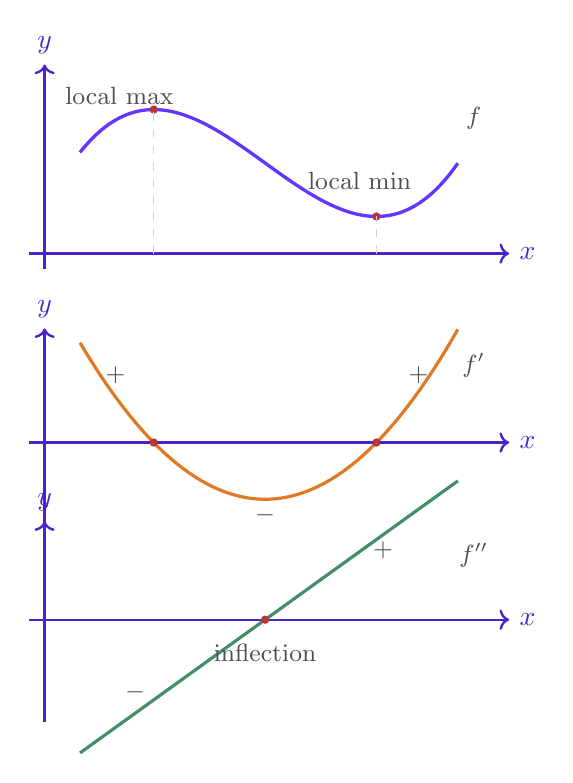
\begin{tikzpicture}[x=1.0cm,y=1.0cm]

% Key x-values
\pgfmathsetmacro{\xa}{1.386}   % local max of f, zero of f'
\pgfmathsetmacro{\xi}{2.800}   % inflection of f, zero of f''
\pgfmathsetmacro{\xb}{4.214}   % local min of f, zero of f'

% =========================
% Top panel: f
% =========================
\begin{scope}[shift={(0,4.4)}]
    \draw[novelPurpleDark, line width=0.85pt, ->] (-0.2,0) -- (5.9,0) node[right] {$x$};
    \draw[novelPurpleDark, line width=0.85pt, ->] (0,-0.2) -- (0,2.4) node[above] {$y$};

    \draw[novelPurple, line width=1.2pt, smooth, samples=260, domain=0.45:5.25]
        plot (\x,{0.12*(\x-2.8)^3 - 0.72*(\x-2.8) + 1.15});

    % key points on f
    \pgfmathsetmacro{\ya}{0.12*(\xa-2.8)^3 - 0.72*(\xa-2.8) + 1.15}
    \pgfmathsetmacro{\yi}{0.12*(\xi-2.8)^3 - 0.72*(\xi-2.8) + 1.15}
    \pgfmathsetmacro{\yb}{0.12*(\xb-2.8)^3 - 0.72*(\xb-2.8) + 1.15}

    \fill[npred] (\xa,\ya) circle (1.5pt);
    \fill[npred] (\xb,\yb) circle (1.5pt);

    \draw[gray!35,dashed] (\xa,0) -- (\xa,\ya);
    \draw[gray!35,dashed] (\xb,0) -- (\xb,\yb);

    \node[text=npgray] at (0.95,2.0) {\small local max};
    \node[text=npgray] at (4.0,0.92) {\small local min};
    \node[text=npgray] at (5.45,1.72) {\small $f$};
\end{scope}

% =========================
% Middle panel: f'
% =========================
\begin{scope}[shift={(0,2.0)}]
    \draw[novelPurpleDark, line width=0.85pt, ->] (-0.2,0) -- (5.9,0) node[right] {$x$};
    \draw[novelPurpleDark, line width=0.85pt, ->] (0,-1.2) -- (0,1.45) node[above] {$y$};

    \draw[nporange, line width=1.15pt, smooth, samples=260, domain=0.45:5.25]
        plot (\x,{0.36*(\x-2.8)^2 - 0.72});

    % zeros of f'
    \fill[npred] (\xa,0) circle (1.5pt);
    \fill[npred] (\xb,0) circle (1.5pt);

    \draw[gray!35,dashed] (\xa,0)--(\xa,{0.36*(\xa-2.8)^2 - 0.72});
    \draw[gray!35,dashed] (\xb,0)--(\xb,{0.36*(\xb-2.8)^2 - 0.72});

    \node[text=npgray] at (0.9,0.86) {\small $+$};
    \node[text=npgray] at (2.8,-0.92) {\small $-$};
    \node[text=npgray] at (4.75,0.86) {\small $+$};
    \node[text=npgray] at (5.45,0.98) {\small $f'$};
\end{scope}

% =========================
% Bottom panel: f''
% =========================
\begin{scope}[shift={(0,-0.25)}]
    \draw[novelPurpleDark, line width=0.85pt, ->] (-0.2,0) -- (5.9,0) node[right] {$x$};
    \draw[novelPurpleDark, line width=0.85pt, ->] (0,-1.3) -- (0,1.25) node[above] {$y$};

    \draw[npgreen, line width=1.15pt, smooth, samples=180, domain=0.45:5.25]
        plot (\x,{0.72*(\x-2.8)});

    % zero of f''
    \fill[npred] (\xi,0) circle (1.5pt);
    \draw[gray!35,dashed] (\xi,0)--(\xi,{0.72*(\xi-2.8)});

    \node[text=npgray] at (1.15,-0.92) {\small $-$};
    \node[text=npgray] at (4.3,0.88) {\small $+$};
    \node[text=npgray] at (2.8,-0.42) {\small inflection};
    \node[text=npgray] at (5.45,0.82) {\small $f''$};
\end{scope}

\end{tikzpicture}
\end{center}
}

\newcommand{\optimizationfigure}{
\begin{center}
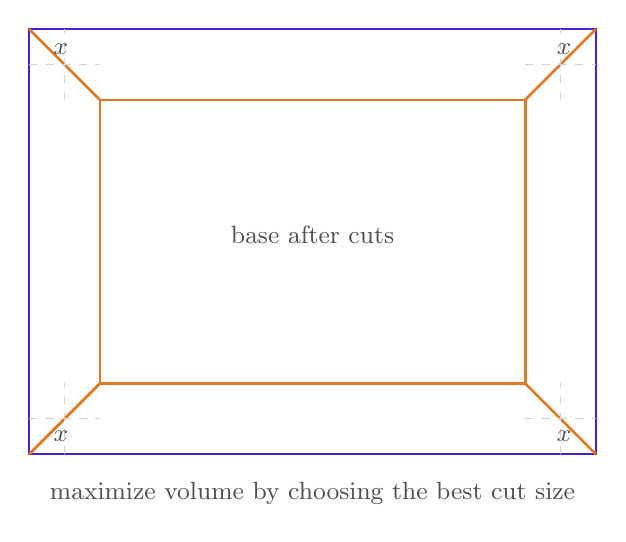
\begin{tikzpicture}[x=0.9cm,y=0.9cm]

    % original sheet
    \draw[novelPurpleDark, line width=0.9pt] (0,0) rectangle (8,6);

    % cut corners
    \draw[nporange, line width=1.0pt] (1,1) rectangle (7,5);

    % corner squares
    \draw[nporange, line width=1.0pt] (0,0)--(1,1);
    \draw[nporange, line width=1.0pt] (8,0)--(7,1);
    \draw[nporange, line width=1.0pt] (0,6)--(1,5);
    \draw[nporange, line width=1.0pt] (8,6)--(7,5);

    % labels x
    \draw[gray!35,dashed] (0,0.5)--(1,0.5);
    \draw[gray!35,dashed] (0.5,0)--(0.5,1);
    \node[text=npgray] at (0.45,0.25) {\small $x$};

    \draw[gray!35,dashed] (7,0.5)--(8,0.5);
    \draw[gray!35,dashed] (7.5,0)--(7.5,1);
    \node[text=npgray] at (7.55,0.25) {\small $x$};

    \draw[gray!35,dashed] (0,5.5)--(1,5.5);
    \draw[gray!35,dashed] (0.5,5)--(0.5,6);
    \node[text=npgray] at (0.45,5.72) {\small $x$};

    \draw[gray!35,dashed] (7,5.5)--(8,5.5);
    \draw[gray!35,dashed] (7.5,5)--(7.5,6);
    \node[text=npgray] at (7.55,5.72) {\small $x$};

    % center labels
    \node[text=npgray] at (4,3.1) {\small base after cuts};
    \node[text=npgray] at (4,-0.55) {\small maximize volume by choosing the best cut size};

\end{tikzpicture}
\end{center}
}

\newcommand{\implicittangentfigure}{
\begin{center}
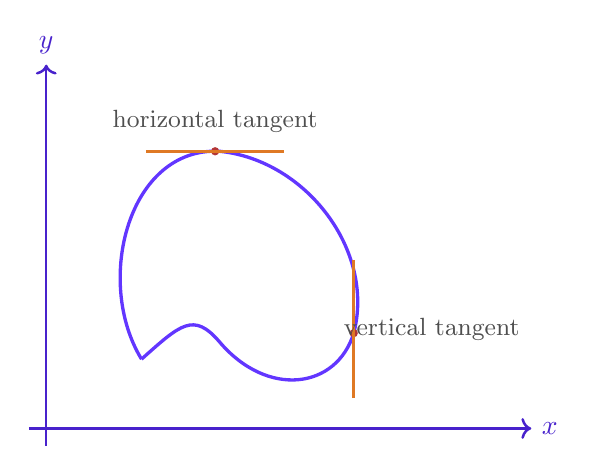
\begin{tikzpicture}[x=1.1cm,y=1.1cm]
    \draw[novelPurpleDark, line width=0.9pt, ->] (-0.2,0) -- (5.6,0) node[right] {$x$};
    \draw[novelPurpleDark, line width=0.9pt, ->] (0,-0.2) -- (0,4.2) node[above] {$y$};

    % implicit-looking loop-ish branch
    \draw[novelPurple, line width=1.2pt]
        (1.1,0.8)
        .. controls (0.55,1.7) and (0.95,3.25) .. (2.0,3.2)
        .. controls (3.0,3.1) and (3.8,2.05) .. (3.55,1.1)
        .. controls (3.35,0.45) and (2.55,0.35) .. (2.0,1.0)
        .. controls (1.7,1.35) and (1.55,1.2) .. (1.1,0.8);

    % horizontal tangent point
    \fill[npred] (1.95,3.2) circle (1.5pt);
    \draw[nporange, line width=1.0pt] (1.15,3.2)--(2.75,3.2);
    \node[text=npgray] at (1.95,3.55) {\small horizontal tangent};

    % vertical tangent point
    \fill[npred] (3.55,1.1) circle (1.5pt);
    \draw[nporange, line width=1.0pt] (3.55,0.35)--(3.55,1.95);
    \node[text=npgray] at (4.45,1.15) {\small vertical tangent};
\end{tikzpicture}
\end{center}
}

% =========================================================
\begin{document}

\begin{titlepage}
\centering
\vspace*{2.0cm}

{\fontsize{28}{32}\selectfont\bfseries\color{novelPurpleDark} AP Calculus AB \& BC\par}
\vspace{0.35cm}
{\fontsize{28}{32}\selectfont\bfseries\color{novelPurpleDark} Unit 5: Analytical Applications of Differentiation\par}



\vspace{1.0cm}

\unitcoverfigure

\vfill

\begin{minipage}{0.84\textwidth}
\begin{notebox}{Design Goals for This Revision}
\begin{itemize}
    \item Preserve the full Unit 5 topic flow from the original PDF and your revised code.
    \item Keep 5.1 and 5.2 strong, but fix the inaccurate figures and strengthen later sections.
    \item Expand 5.4 through 5.9 so the chapter feels complete, not outline-level.
    \item Replace weak or underdeveloped visuals with cleaner, more accurate TikZ figures.
    \item Make the optimization and implicit-relation sections actually useful for teaching.
\end{itemize}
\end{notebox}
\end{minipage}

\vfill

{\large\textbf{Novel Prep Learning Center}}\\[0.25em]
{\large J. Z}

\end{titlepage}

\tableofcontents
\newpage

\setcounter{section}{4}
\section{Analytical Applications of Differentiation}

\begin{theorybox}{Big Idea}
Unit 5 turns derivative information into conclusions about the shape and behavior of a function.
\[
\text{derivative} \longrightarrow \text{increase/decrease} \longrightarrow \text{extrema / concavity} \longrightarrow \text{graph / optimization}
\]
\end{theorybox}

\begin{notebox}{Teaching Philosophy for This Unit}
Students should not see derivative tests as isolated tricks.  
They should understand that the derivative is a language for describing:
\begin{itemize}
    \item where a function rises or falls,
    \item where it reaches a high or low point,
    \item how it bends,
    \item and how to optimize real quantities.
\end{itemize}
\end{notebox}

\apcheckpoint{
The chapter naturally unfolds in four layers:
\begin{itemize}
    \item \textbf{Existence theorems:} Rolle’s Theorem, MVT, EVT.
    \item \textbf{Local behavior:} critical numbers, first derivative test, second derivative test.
    \item \textbf{Global shape:} graph sketching and $f,f',f''$ relationships.
    \item \textbf{Applications:} optimization and implicit-relation behavior.
\end{itemize}
}

% =========================================================
\unitchapter{Rolle’s Theorem and the Mean Value Theorem}

\unitsubtopic{Rolle’s Theorem}

\begin{theorybox}{Theorem 5.1.1 --- Rolle’s Theorem}
Let $f$ be continuous on the closed interval $[a,b]$ and differentiable on the open interval $(a,b)$.  
If
\[
f(a)=f(b),
\]
then there exists at least one number $c\in(a,b)$ such that
\[
f'(c)=0.
\]
\end{theorybox}

\begin{notebox}{Interpretation}
If a smooth curve starts and ends at the same height, then at some interior point it must have a horizontal tangent.
\end{notebox}

\rollefigure

\example{Illustrating Rolle’s Theorem}
Find the two $x$-intercepts of
\[
f(x)=x^2-3x+2
\]
and show that $f'(x)=0$ at some point between the intercepts.

\solution
Set $f(x)=0$:
\[
x^2-3x+2=0
\quad\Longrightarrow\quad
(x-1)(x-2)=0.
\]
So the $x$-intercepts are
\[
x=1,\quad x=2.
\]
Because $f$ is differentiable everywhere and $f(1)=f(2)=0$, Rolle’s Theorem guarantees a value $c\in(1,2)$ such that $f'(c)=0$.

Differentiate:
\[
f'(x)=2x-3.
\]
Set equal to zero:
\[
2x-3=0 \Rightarrow x=\frac32.
\]
Since
\[
\frac32\in(1,2),
\]
this verifies Rolle’s Theorem.

\unitsubtopic{Mean Value Theorem}

\begin{theorybox}{Theorem 5.1.2 --- Mean Value Theorem}
If $f$ is continuous on $[a,b]$ and differentiable on $(a,b)$, then there exists a number $c\in(a,b)$ such that
\[
f'(c)=\frac{f(b)-f(a)}{b-a}.
\]
\end{theorybox}

\mvttangentfigure

\example{Finding a tangent line parallel to a secant line}
For
\[
f(x)=5-\frac{4}{x},
\]
find all values of $c$ in the open interval $(1,4)$ such that
\[
f'(c)=\frac{f(4)-f(1)}{4-1}.
\]

\solution
First compute the secant slope:
\[
f(1)=5-4=1,\qquad f(4)=5-1=4.
\]
So
\[
\frac{f(4)-f(1)}{4-1}=\frac{4-1}{3}=1.
\]
Differentiate:
\[
f'(x)=\frac{4}{x^2}.
\]
Set equal to $1$:
\[
\frac{4}{x^2}=1
\quad\Longrightarrow\quad
x^2=4
\quad\Longrightarrow\quad
x=\pm 2.
\]
Only $x=2$ lies in $(1,4)$, so
\[
\boxed{c=2.}
\]

% =========================================================
\unitchapter{Extrema on an Interval}

\unitsubtopic{Extrema of a Function}

\begin{theorybox}{Definition 5.2.1 --- Extrema}
Let $f$ be defined on an interval $I$ containing $c$.
\begin{itemize}
    \item $f(c)$ is a \textbf{minimum} of $f$ on $I$ if $f(c)\le f(x)$ for all $x\in I$.
    \item $f(c)$ is a \textbf{maximum} of $f$ on $I$ if $f(c)\ge f(x)$ for all $x\in I$.
\end{itemize}
The minimum and maximum values of a function on an interval are called its \textbf{extrema}.  
Absolute maxima and minima are also called \textbf{global extrema}.
\end{theorybox}

\begin{notebox}{Why This Matters}
Students often mix up \emph{local} and \emph{absolute} extrema.  
A local extremum only compares nearby values, while an absolute extremum compares all values on the interval.
\end{notebox}

\extremaoverviewfigure

\begin{theorybox}{Theorem 5.2.1 --- Extreme Value Theorem}
If $f$ is continuous on a closed interval $[a,b]$, then $f$ has both a minimum and a maximum on $[a,b]$.
\end{theorybox}

\begin{notebox}{Important Consequence}
The Extreme Value Theorem guarantees \textbf{existence}, but it does not tell us \emph{where} the extrema occur.  
They may occur at:
\begin{itemize}
    \item an interior critical number, or
    \item one of the endpoints.
\end{itemize}
\end{notebox}

\localvsabsolutefigure

\begin{summarybox}{Absolute vs. Relative Extrema}
\begin{itemize}
    \item A \textbf{relative (local) maximum} is the highest value in a small neighborhood.
    \item A \textbf{relative (local) minimum} is the lowest value in a small neighborhood.
    \item An \textbf{absolute maximum} is the highest value on the entire interval.
    \item An \textbf{absolute minimum} is the lowest value on the entire interval.
\end{itemize}
\end{summarybox}

\unitsubtopic{Relative Extrema and Critical Numbers}

\begin{theorybox}{Definition 5.2.2 --- Relative Extrema}
If $f(c)$ is a maximum or minimum on some open interval around $c$, then $f(c)$ is called a \textbf{relative} (or \textbf{local}) maximum or minimum.
\end{theorybox}

\begin{theorybox}{Definition 5.2.3 --- Critical Number}
A number $c$ in the domain of $f$ is a \textbf{critical number} if
\[
f'(c)=0
\]
or if $f'(c)$ does not exist.
\end{theorybox}

\criticalfigure

\begin{theorybox}{Theorem 5.2.2 --- Relative Extrema Occur Only at Critical Numbers}
If $f$ has a relative maximum or relative minimum at $x=c$, then $c$ is a critical number of $f$.
\end{theorybox}

\begin{notebox}{Important Warning}
A critical number does \textbf{not} automatically mean there is an extremum there.  
It is only a \emph{candidate}. Later derivative tests help determine whether it is actually a max, a min, or neither.
\end{notebox}

\example{Reading local and absolute extrema from a graph}
Consider
\[
f(x)=3x^4-16x^3+18x^2,\qquad -1\le x\le 4.
\]
Describe the relative and absolute extrema.

\solution
From the original note:
\begin{itemize}
    \item $f(1)=5$ is a local maximum.
    \item $f(0)=0$ is a local minimum.
    \item $f(3)=-27$ is both a local and absolute minimum.
    \item $f(-1)=37$ is the absolute maximum on the interval.
\end{itemize}

\unitsubtopic{Finding Extrema on a Closed Interval}

\begin{notebox}{Guidelines for Finding Extrema on a Closed Interval}
To find extrema of a continuous function $f$ on $[a,b]$:
\begin{enumerate}
    \item Find all critical numbers in $(a,b)$.
    \item Evaluate $f$ at each critical number.
    \item Evaluate $f$ at each endpoint.
    \item Compare all resulting values.
\end{enumerate}
The least value is the absolute minimum, and the greatest value is the absolute maximum.
\end{notebox}

\closedintervalextremafigure

\begin{summarybox}{Closed Interval Strategy}
On a closed interval, the complete candidate list is:
\[
\boxed{\text{left endpoint} \;+\; \text{all critical numbers in the interior} \;+\; \text{right endpoint}.}
\]
This is why endpoint checking is essential.
\end{summarybox}

\example{Find extrema on a closed interval}
Find the extrema of
\[
f(x)=3x^4-4x^3
\]
on the interval $[-1,2]$.

\solution
Differentiate:
\[
f'(x)=12x^3-12x^2=12x^2(x-1).
\]
Critical numbers in $(-1,2)$:
\[
x=0,\quad x=1.
\]
Evaluate:
\[
f(-1)=7,\qquad f(0)=0,\qquad f(1)=-1,\qquad f(2)=16.
\]
Compare these values:
\[
-1<0<7<16.
\]
So the absolute minimum is
\[
\boxed{f(1)=-1}
\]
and the absolute maximum is
\[
\boxed{f(2)=16.}
\]

% =========================================================
\unitchapter{Increasing and Decreasing Functions}

\begin{theorybox}{Definition 5.3.1 --- Increasing and Decreasing Functions}
A function $f$ is increasing on an interval if $x_1<x_2$ implies $f(x_1)<f(x_2)$.  
A function $f$ is decreasing on an interval if $x_1<x_2$ implies $f(x_1)>f(x_2)$.
\end{theorybox}

\begin{theorybox}{Theorem 5.3.1 --- Test for Increasing and Decreasing Functions}
If $f$ is continuous on $[a,b]$ and differentiable on $(a,b)$:
\begin{itemize}
    \item If $f'(x)>0$ for all $x\in(a,b)$, then $f$ is increasing on $[a,b]$.
    \item If $f'(x)<0$ for all $x\in(a,b)$, then $f$ is decreasing on $[a,b]$.
    \item If $f'(x)=0$ for all $x\in(a,b)$, then $f$ is constant on $[a,b]$.
\end{itemize}
\end{theorybox}

\incdecfigure

\example{Intervals on which $f$ is increasing or decreasing}
Find the open intervals on which
\[
f(x)=x^3-\frac32x^2
\]
is increasing or decreasing.

\solution
Differentiate:
\[
f'(x)=3x^2-3x=3x(x-1).
\]
Critical numbers:
\[
x=0,\quad x=1.
\]
Test intervals:

\[
\begin{array}{c|c|c|c}
\text{Interval} & (-\infty,0) & (0,1) & (1,\infty)\\
\hline
\text{Test value} & -1 & \frac12 & 2\\
\hline
f'(x) & >0 & <0 & >0
\end{array}
\]

So $f$ is:
\[
\boxed{\text{increasing on }(-\infty,0)\cup(1,\infty)}
\]
and
\[
\boxed{\text{decreasing on }(0,1).}
\]

\begin{notebox}{Guidelines for Finding Intervals}
\begin{enumerate}
    \item Find critical numbers.
    \item Use them to split the number line into intervals.
    \item Test the sign of $f'$ in each interval.
    \item Interpret the sign of $f'$.
\end{enumerate}
\end{notebox}

% =========================================================
\unitchapter{The First Derivative Test}

\begin{theorybox}{Theorem 5.4.1 --- The First Derivative Test}
Let $c$ be a critical number of a function $f$ that is continuous on an open interval containing $c$. If $f$ is differentiable except possibly at $c$, then:
\begin{itemize}
    \item If $f'$ changes from negative to positive at $c$, then $f$ has a relative minimum at $c$.
    \item If $f'$ changes from positive to negative at $c$, then $f$ has a relative maximum at $c$.
    \item If $f'$ does not change sign, then $f(c)$ is neither a relative minimum nor a relative maximum.
\end{itemize}
\end{theorybox}

\begin{notebox}{Why This Test Matters}
The First Derivative Test is stronger than simply locating critical numbers.  
It classifies what actually happens at those critical numbers by looking at the sign of $f'$ on each side.
\end{notebox}

\firstderivfigure

\begin{summarybox}{Sign-Chart Logic}
\[
(-)\to (+)\Rightarrow \text{relative minimum}
\]
\[
(+)\to (-)\Rightarrow \text{relative maximum}
\]
\[
(-)\to (-)\text{ or }(+)\to (+)\Rightarrow \text{neither}
\]
\end{summarybox}
\newpage
\example{Applying the First Derivative Test}
Find the relative extrema of
\[
f(x)=\frac12x-\sin x
\]
in the interval $(0,2\pi)$.

\solution
Differentiate:
\[
f'(x)=\frac12-\cos x.
\]
Set equal to zero:
\[
\frac12-\cos x=0
\quad\Longrightarrow\quad
\cos x=\frac12.
\]
So the critical numbers are
\[
x=\frac{\pi}{3},\qquad x=\frac{5\pi}{3}.
\]

Check signs of $f'$:
\[
\begin{array}{c|c|c|c}
\text{Interval} & \left(0,\frac{\pi}{3}\right) & \left(\frac{\pi}{3},\frac{5\pi}{3}\right) & \left(\frac{5\pi}{3},2\pi\right)\\
\hline
f'(x) & <0 & >0 & <0
\end{array}
\]

So:
\begin{itemize}
    \item relative minimum at $x=\frac{\pi}{3}$,
    \item relative maximum at $x=\frac{5\pi}{3}$.
\end{itemize}

\example{A rational-function example}
Find the relative extrema of
\[
f(x)=\frac{x^4+1}{x^2}.
\]

\solution
Rewrite:
\[
f(x)=x^2+x^{-2}.
\]
Differentiate:
\[
f'(x)=2x-2x^{-3}
=\frac{2(x^4-1)}{x^3}
=\frac{2(x^2+1)(x-1)(x+1)}{x^3}.
\]
Critical numbers are
\[
x=-1,\quad x=1.
\]
Also $x=0$ is not in the domain, so it separates intervals.

A sign chart gives:
\[
(-\infty,-1),\quad (-1,0),\quad (0,1),\quad (1,\infty).
\]
From the sign changes:
\begin{itemize}
    \item $x=-1$ is a relative minimum,
    \item $x=1$ is a relative minimum,
    \item no relative maximum occurs.
\end{itemize}

% =========================================================
\unitchapter{Determine Absolute Extrema from Candidates}

\noindent
\textbf{Why This Section Matters}

\smallskip

Students often learn how to find critical numbers and how to classify local extrema, but AP-style questions frequently ask a different question:
\emph{which candidate actually gives the absolute maximum or absolute minimum on a closed interval?}
This section builds the bridge from local behavior to global conclusions.
Later on, the same exact idea will appear again in optimization, particle motion, and graph-analysis questions.

\vspace{0.75em}

\begin{theorybox}{Core Principle of 5.5}
For a continuous function on a closed interval \([a,b]\), the candidates for absolute extrema are:
\begin{enumerate}
    \item all critical numbers in the interior \((a,b)\),
    \item the endpoints \(a\) and \(b\).
\end{enumerate}
\end{theorybox}

\begin{center}
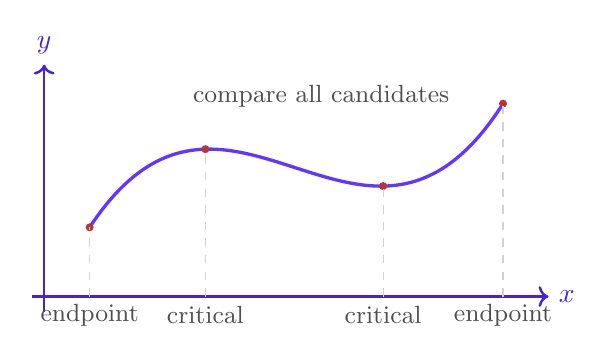
\begin{tikzpicture}[x=1.05cm,y=0.95cm]
    % axes
    \draw[novelPurpleDark, line width=0.9pt, ->] (-0.15,0) -- (6.1,0) node[right] {$x$};
    \draw[novelPurpleDark, line width=0.9pt, ->] (0,-0.2) -- (0,3.1) node[above] {$y$};

    % curve
    \draw[novelPurple, line width=1.2pt, smooth, samples=220, domain=0.55:5.55]
        plot (\x,{0.11*(\x-1.2)*(\x-3.1)*(\x-4.8)+1.7});

    % candidate points
    \pgfmathsetmacro{\xa}{0.55}
    \pgfmathsetmacro{\xcOne}{1.95}
    \pgfmathsetmacro{\xcTwo}{4.10}
    \pgfmathsetmacro{\xb}{5.55}
    \pgfmathsetmacro{\ya}{0.11*(\xa-1.2)*(\xa-3.1)*(\xa-4.8)+1.7}
    \pgfmathsetmacro{\ycOne}{0.11*(\xcOne-1.2)*(\xcOne-3.1)*(\xcOne-4.8)+1.7}
    \pgfmathsetmacro{\ycTwo}{0.11*(\xcTwo-1.2)*(\xcTwo-3.1)*(\xcTwo-4.8)+1.7}
    \pgfmathsetmacro{\yb}{0.11*(\xb-1.2)*(\xb-3.1)*(\xb-4.8)+1.7}

    \fill[npred] (\xa,\ya) circle (1.45pt);
    \fill[npred] (\xcOne,\ycOne) circle (1.45pt);
    \fill[npred] (\xcTwo,\ycTwo) circle (1.45pt);
    \fill[npred] (\xb,\yb) circle (1.45pt);

    \draw[gray!35,dashed] (\xa,0)--(\xa,\ya);
    \draw[gray!35,dashed] (\xcOne,0)--(\xcOne,\ycOne);
    \draw[gray!35,dashed] (\xcTwo,0)--(\xcTwo,\ycTwo);
    \draw[gray!35,dashed] (\xb,0)--(\xb,\yb);

    \node[text=npgray] at (\xa,-0.25) {\small endpoint};
    \node[text=npgray] at (\xcOne,-0.25) {\small critical};
    \node[text=npgray] at (\xcTwo,-0.25) {\small critical};
    \node[text=npgray] at (\xb,-0.25) {\small endpoint};
    \node[text=npgray] at (3.35,2.68) {\small compare all candidates};
\end{tikzpicture}
\end{center}

\begin{summarybox}{Absolute Extrema Checklist}
\begin{enumerate}
    \item Confirm the interval is closed.
    \item Find all critical numbers in the open interval.
    \item Evaluate the original function at every critical number and every endpoint.
    \item Compare the resulting function values.
    \item State both the \emph{value} and the \emph{x-location} of the absolute maximum and absolute minimum.
\end{enumerate}
\end{summarybox}
\newpage
\unitsubtopic{Why Endpoints Matter}

\noindent
A very common student error is to stop after finding critical numbers.
That only finds \emph{interior candidates}.
On a closed interval, an endpoint can still produce the largest or smallest value.

\begin{center}
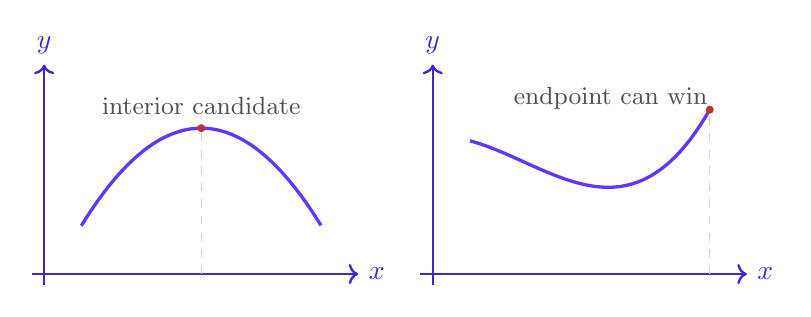
\begin{tikzpicture}[x=1.05cm,y=0.95cm]
    \begin{scope}[shift={(0,0)}]
        \draw[novelPurpleDark, line width=0.85pt, ->] (-0.15,0)--(3.8,0) node[right] {$x$};
        \draw[novelPurpleDark, line width=0.85pt, ->] (0,-0.15)--(0,2.8) node[above] {$y$};
        \draw[novelPurple, line width=1.2pt, smooth, samples=180, domain=0.45:3.35]
            plot (\x,{1.95-0.62*(\x-1.9)^2});
        \fill[npred] (1.9,1.95) circle (1.45pt);
        \draw[gray!35,dashed] (1.9,0)--(1.9,1.95);
        \node[text=npgray] at (1.9,2.25) {\small interior candidate};
    \end{scope}

    \begin{scope}[shift={(4.7,0)}]
        \draw[novelPurpleDark, line width=0.85pt, ->] (-0.15,0)--(3.8,0) node[right] {$x$};
        \draw[novelPurpleDark, line width=0.85pt, ->] (0,-0.15)--(0,2.8) node[above] {$y$};
        \draw[novelPurple, line width=1.2pt, smooth, samples=180, domain=0.45:3.35]
            plot (\x,{0.16*(\x-1.1)^3-0.5*(\x-1.1)+1.5});
        \pgfmathsetmacro{\yr}{0.16*(3.35-1.1)^3-0.5*(3.35-1.1)+1.5}
        \fill[npred] (3.35,\yr) circle (1.45pt);
        \draw[gray!35,dashed] (3.35,0)--(3.35,\yr);
        \node[text=npgray] at (2.15,2.35) {\small endpoint can win};
    \end{scope}
\end{tikzpicture}
\end{center}

\begin{notebox}{Important Distinction}
A relative maximum is not automatically the absolute maximum, and a relative minimum is not automatically the absolute minimum.
Absolute extrema are decided only after comparing \emph{all candidates} on the interval.
\end{notebox}

\unitsubtopic{Worked Example: Algebraic Function on a Closed Interval}

\example{Find absolute extrema of a polynomial on a closed interval}
Find the absolute maximum value and the absolute minimum value of
\[
f(x)=x^3-3x^2+1
\]
on the interval
\[
\left[-\frac12,4\right].
\]

\solution

\textbf{Step 1: Find critical numbers in the interior.}

\[
f'(x)=3x^2-6x=3x(x-2).
\]
So the critical numbers are
\[
x=0,\qquad x=2.
\]
Both lie in the interval \(\left[-\frac12,4\right]\).

\textbf{Step 2: Evaluate the function at all candidates.}

The candidates are
\[
-\frac12,\quad 0,\quad 2,\quad 4.
\]

Now compute:
\[
f\left(-\frac12\right)=\left(-\frac12\right)^3-3\left(-\frac12\right)^2+1
=-\frac18-\frac34+1=\frac18,
\]
\[
f(0)=1,
\]
\[
f(2)=8-12+1=-3,
\]
\[
f(4)=64-48+1=17.
\]

\textbf{Step 3: Compare the values.}

\[
\frac18,\quad 1,\quad -3,\quad 17.
\]

Therefore,
\[
\boxed{\text{absolute minimum value }=-3 \text{ at } x=2}
\]
and
\[
\boxed{\text{absolute maximum value }=17 \text{ at } x=4.}
\]

\begin{summarybox}{What This Example Teaches}
One absolute extremum came from a critical number \((x=2)\), but the other came from an endpoint \((x=4)\).
That is exactly why endpoints must always be checked.
\end{summarybox}
\newpage
\unitsubtopic{Different Function Families, Same Logic}

\noindent
This topic is especially important because the same checklist works across many different function families:
polynomials, rational functions, trigonometric functions, and exponential functions.
The derivative algebra changes, but the absolute-extrema structure does not.

\begin{theorybox}{Same Strategy, Different Algebra}
No matter which function family appears, the structure is always the same:
\begin{enumerate}
    \item differentiate,
    \item solve for interior critical numbers,
    \item keep only those that lie in the interval,
    \item evaluate the original function at all candidates,
    \item compare actual function values.
\end{enumerate}
\end{theorybox}

\example{Exponential example}
Let
\[
g(x)=xe^{2x}, \qquad -1\le x\le 1.
\]
Find the absolute extrema.

\solution
Differentiate using the product rule:
\[
g'(x)=e^{2x}+2xe^{2x}=e^{2x}(1+2x).
\]
Since \(e^{2x}>0\) for all \(x\), critical numbers occur when
\[
1+2x=0 \Rightarrow x=-\frac12.
\]
The candidates are
\[
-1,\quad -\frac12,\quad 1.
\]
Now evaluate:
\[
g(-1)=-e^{-2},
\]
\[
g\left(-\frac12\right)=-\frac12 e^{-1},
\]
\[
g(1)=e^2.
\]
Comparing these values,
\[
\boxed{\text{absolute minimum at }x=-\frac12}
\]
and
\[
\boxed{\text{absolute maximum at }x=1.}
\]

\example{Trig example}
Find the absolute extrema of
\[
f(x)=\sin\left(x+\frac{\pi}{4}\right)
\]
on
\[
\left[0,\frac{7\pi}{4}\right].
\]

\solution
Differentiate:
\[
f'(x)=\cos\left(x+\frac{\pi}{4}\right).
\]
Set equal to zero:
\[
\cos\left(x+\frac{\pi}{4}\right)=0.
\]
So
\[
x+\frac{\pi}{4}=\frac{\pi}{2},\ \frac{3\pi}{2},\ \frac{5\pi}{2},\dots
\]
Hence
\[
x=\frac{\pi}{4},\quad x=\frac{5\pi}{4}
\]
are the critical numbers in the interval.

Now evaluate all candidates:
\[
f(0)=\sin\left(\frac{\pi}{4}\right)=\frac{\sqrt2}{2},
\]
\[
f\left(\frac{\pi}{4}\right)=\sin\left(\frac{\pi}{2}\right)=1,
\]
\[
f\left(\frac{5\pi}{4}\right)=\sin\left(\frac{3\pi}{2}\right)=-1,
\]
\[
f\left(\frac{7\pi}{4}\right)=\sin(2\pi)=0.
\]

Therefore,
\[
\boxed{\text{absolute maximum value }=1 \text{ at } x=\frac{\pi}{4}}
\]
and
\[
\boxed{\text{absolute minimum value }=-1 \text{ at } x=\frac{5\pi}{4}.}
\]
\newpage
\unitsubtopic{Reading Absolute Extrema from a Graph of \texorpdfstring{$f'$}{f'}}

\noindent
A more advanced version of this skill appears when a problem gives the graph of \(f'\) instead of a formula for \(f\).
In that setting, students cannot just look for sign changes.
They must think globally about how much \(f\) has increased or decreased across the entire interval.

\begin{center}
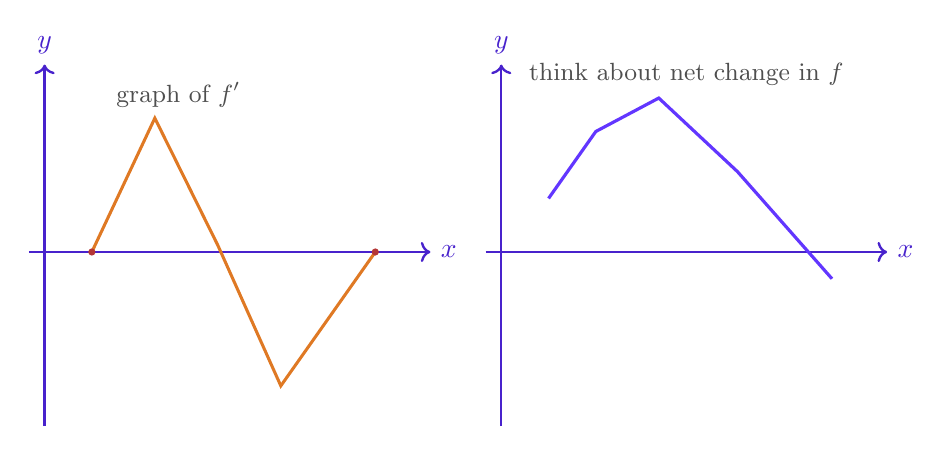
\begin{tikzpicture}[x=1.0cm,y=0.85cm]
    \begin{scope}[shift={(0,0)}]
        \draw[novelPurpleDark, line width=0.85pt, ->] (-0.2,0)--(4.9,0) node[right] {$x$};
        \draw[novelPurpleDark, line width=0.85pt, ->] (0,-2.6)--(0,2.8) node[above] {$y$};
        \draw[nporange, line width=1.1pt, smooth] (0.6,0)--(1.4,2.0)--(2.2,0.1)--(3.0,-2.0)--(4.2,0);
        \fill[npred] (0.6,0) circle (1.3pt);
        \fill[npred] (4.2,0) circle (1.3pt);
        \node[text=npgray] at (1.7,2.35) {\small graph of $f'$};
    \end{scope}

    \begin{scope}[shift={(5.8,0)}]
        \draw[novelPurpleDark, line width=0.85pt, ->] (-0.2,0)--(4.9,0) node[right] {$x$};
        \draw[novelPurpleDark, line width=0.85pt, ->] (0,-2.6)--(0,2.8) node[above] {$y$};
        \draw[novelPurple, line width=1.15pt, smooth] (0.6,0.8)--(1.2,1.8)--(2.0,2.3)--(3.0,1.2)--(4.2,-0.4);
        \node[text=npgray] at (2.35,2.65) {\small think about net change in $f$};
    \end{scope}
\end{tikzpicture}
\end{center}

\begin{notebox}{Key Idea When a Graph of \texorpdfstring{$f'$}{f'} Is Given}
To locate absolute extrema of \(f\) on a closed interval using a graph of \(f'\):
\begin{itemize}
    \item identify candidate x-values from endpoints and where \(f'=0\) or \(f'\) is undefined,
    \item then decide which x-value gives the greatest or least \emph{accumulated change} in \(f\),
    \item not just where \(f'\) switches sign.
\end{itemize}
A sign change gives local information; absolute extrema require global comparison.
\end{notebox}

\example{Reasoning from a graph of \texorpdfstring{$f'$}{f'}}
Suppose \(f'\) is positive on most of \([-2,0]\) and negative on most of \((0,3]\), with only one sign change at \(x=0\).
What is the strongest candidate for the absolute maximum of \(f\)?

\solution
If \(f'>0\) up to \(x=0\), then \(f\) is increasing toward \(x=0\).
If \(f'<0\) after \(x=0\), then \(f\) decreases after that point.
So \(x=0\) is the strongest candidate for the absolute maximum.

However, on a full closed-interval problem, the endpoints must still be checked before making a final conclusion.
\newpage
\unitsubtopic{Extensions: Piecewise Functions and Motion}

\noindent
This topic is much more important than it first appears because the same absolute-extrema logic shows up in many later problem types:
piecewise functions, particle motion, and applied derivative problems.

\begin{theorybox}{Where 5.5 Shows Up Later}
The same closed-interval candidate method will appear in:
\begin{itemize}
    \item optimization problems,
    \item minimum and maximum velocity questions,
    \item farthest-right / farthest-left particle position questions,
    \item and maximum acceleration questions built from derivatives of motion functions.
\end{itemize}
\end{theorybox}

\example{Motion extension: minimum velocity}
A particle moves along the \(y\)-axis so that its velocity at time \(t\), \(0\le t\le 6\), is given by
\[
v(t)=2(t-2)(t-5).
\]
Find the minimum velocity.

\solution
Differentiate:
\[
v'(t)=2(t-5)+2(t-2)=4t-14.
\]
Set equal to zero:
\[
4t-14=0 \Rightarrow t=\frac{7}{2}.
\]
Now check all candidates:
\[
t=0,\quad t=\frac72,\quad t=6.
\]
Evaluate:
\[
v(0)=2(-2)(-5)=20,
\]
\[
v\left(\frac72\right)=2\left(\frac32\right)\left(-\frac32\right)=-\frac92,
\]
\[
v(6)=2(4)(1)=8.
\]
So the minimum velocity is
\[
\boxed{-\frac92.}
\]

\example{Piecewise extension}
Consider
\[
f(x)=
\begin{cases}
x^2, & 0\le x<1,\\
0, & 1\le x\le 2.
\end{cases}
\]
What is the absolute minimum value of \(f\) on \([0,2]\)?

\solution
For \(0\le x<1\), we have \(x^2\ge 0\).
For \(1\le x\le 2\), the function is identically \(0\).
So the smallest function value is
\[
\boxed{0.}
\]
In fact, that absolute minimum is attained at every point in \([1,2]\), and also at \(x=0\).

\begin{summarybox}{Why 5.5 Is Foundational}
This chapter is a foundation for later units because the exact same logic appears in:
\begin{itemize}
    \item optimization,
    \item particle motion,
    \item graph interpretation from derivatives,
    \item and later applied free-response questions.
\end{itemize}
Students who truly understand 5.5 stop treating extrema as a memorized procedure and start seeing them as a comparison problem across all legitimate candidates.
\end{summarybox}

\begin{practicebox}{Guided Practice for 5.5}
\begin{enumerate}
    \item Find the absolute extrema of \(f(x)=1+(x+1)^2\) on \([-2,5]\).
    \item Find the absolute extrema of \(f(x)=\dfrac{x}{x^2+1}\) on \([-2,2]\).
    \item Find the absolute extrema of \(f(x)=\sin\left(x+\dfrac{\pi}{4}\right)\) on \(\left[0,\dfrac{7\pi}{4}\right]\).
    \item Explain why a function can have no interior critical numbers and still have an absolute maximum on a closed interval.
    \item Explain why a local maximum is only a candidate for an absolute maximum.
\end{enumerate}
\end{practicebox}



% =========================================================
\unitchapter{Concavity and the Second Derivative Test}

\unitsubtopic{Concavity}

\begin{theorybox}{Concavity}
\begin{itemize}
    \item If $f''(x)>0$, the graph of $f$ is concave up.
    \item If $f''(x)<0$, the graph of $f$ is concave down.
\end{itemize}
\end{theorybox}

\concavityfigure

\unitsubtopic{Points of Inflection}

\begin{theorybox}{Point of Inflection}
A point of inflection occurs where the concavity changes.
\end{theorybox}

\unitsubtopic{The Second Derivative Test}

\begin{theorybox}{Theorem 5.5.3 --- Second Derivative Test}
Suppose $f'(c)=0$ and $f''$ exists near $c$.
\begin{itemize}
    \item If $f''(c)>0$, then $f$ has a relative minimum at $c$.
    \item If $f''(c)<0$, then $f$ has a relative maximum at $c$.
    \item If $f''(c)=0$, the test fails.
\end{itemize}
\end{theorybox}

\example{Using the Second Derivative Test}
Find the relative extrema of
\[
f(x)=-3x^5+5x^3.
\]

\solution
Differentiate:
\[
f'(x)=-15x^4+15x^2=15x^2(1-x^2).
\]
Critical numbers:
\[
x=-1,\quad x=0,\quad x=1.
\]
Second derivative:
\[
f''(x)=-60x^3+30x=30x(1-2x^2).
\]
Evaluate:
\[
f''(-1)>0,\qquad f''(0)=0,\qquad f''(1)<0.
\]
So:
\begin{itemize}
    \item relative minimum at $(-1,-2)$,
    \item test fails at $(0,0)$,
    \item relative maximum at $(1,2)$.
\end{itemize}

% =========================================================
\unitchapter{Sketching Graphs of Functions and Their Derivatives}

% =========================================================
% Intro (NO BOX)
% =========================================================

\noindent
\textbf{Why Graph Sketching Matters}

\smallskip

Graph sketching is where many separate derivative ideas come together. 
Students are no longer answering isolated questions like 
“Where is $f$ increasing?” or “Where is $f$ concave up?”.
Instead, they must combine all of that information into one coherent picture.

\vspace{0.75em}

% =========================================================
% Core checklist (ONLY MAIN BOX)
% =========================================================

\begin{theorybox}{Guidelines for Sketching a Curve}
To sketch $y=f(x)$, check:
\begin{enumerate}
    \item domain,
    \item intercepts,
    \item symmetry,
    \item asymptotes,
    \item intervals of increase or decrease,
    \item local extrema,
    \item concavity and inflection points,
    \item end behavior.
\end{enumerate}
\end{theorybox}



% =========================================================
% Roadmap figure
% =========================================================

\graphroadmapfigure



% =========================================================
% Skeleton (NO BOX)
% =========================================================

\noindent
\textbf{A Good Sketch Starts with the Skeleton}

\vspace{0.4em}

\begin{adjustwidth}{1.5em}{0em}
\begin{itemize}
    \item First locate where the function is allowed to exist.
    \item Then mark intercepts and asymptotes.
    \item Then use $f'$ to determine shape from left to right.
    \item Then use $f''$ to refine concavity.
    \item Finally connect everything smoothly.
\end{itemize}
\end{adjustwidth}

\vspace{1em}

% =========================================================
% Table instead of box (HIGH-END LOOK)
% =========================================================

\unitsubtopic{What Each Ingredient Tells You}

\begin{center}
\renewcommand{\arraystretch}{1.4}
\begin{tabular}{p{4cm} p{9cm}}
\toprule
\textbf{Information} & \textbf{What it tells you about the graph} \\
\midrule
Domain & Where the graph can exist \\
Intercepts & Where the graph crosses the axes \\
Symmetry & Reduces work and improves accuracy \\
Asymptotes & Long-term or near-discontinuity behavior \\
$f'(x)$ & Increasing/decreasing and relative extrema \\
$f''(x)$ & Concavity and inflection points \\
End behavior & Behavior as $x\to\pm\infty$ \\
\bottomrule
\end{tabular}
\end{center}

\vspace{1em}

% =========================================================
% Important principle (ONLY SECOND BOX)
% =========================================================

\begin{notebox}{Important Principle}
Do not try to “freehand guess” the graph first.  
Instead, let each piece of information narrow the possibilities until the graph is essentially forced.
\end{notebox}

\vspace{1em}

% =========================================================
% Example with full logic
% =========================================================

\unitsubtopic{Worked Example: A Rational Function}

\example{Using a full checklist}
Sketch the behavior of
\[
f(x)=\frac{x}{x^2-1}.
\]

\solution

\textbf{Step 1: Domain}

\[
x^2-1\ne0 \quad \Rightarrow \quad x\ne \pm1
\]

\textbf{Step 2: Intercepts}

\[
x=0 \Rightarrow (0,0)
\]

\textbf{Step 3: Symmetry}

\[
f(-x)=-f(x) \Rightarrow \text{odd symmetry}
\]

\textbf{Step 4: Asymptotes}

\[
x=\pm1 \quad \text{(vertical)}, \qquad y=0 \quad \text{(horizontal)}
\]

\rationalsketchfigure

\textbf{Step 5: Increasing/Decreasing}

\[
f'(x)=\frac{-x^2-1}{(x^2-1)^2}<0
\]

So $f$ is decreasing on all intervals.

\textbf{Step 6: Concavity}

\[
f''(x)=\frac{2x(x^2+3)}{(x^2-1)^3}
\]

Sign analysis gives concavity changes at $x=0$.

\textbf{Step 7: Final Graph}

Combine:
\begin{itemize}
    \item asymptotes,
    \item symmetry,
    \item monotonic decrease,
    \item inflection at $(0,0)$.
\end{itemize}

\vspace{0.5em}
\newpage
\begin{summarybox}{Final Behavior of $\frac{x}{x^2-1}$}
\begin{itemize}
    \item Domain: $x\ne\pm1$
    \item Intercept: $(0,0)$
    \item Odd symmetry
    \item Decreasing everywhere
    \item Inflection at $(0,0)$
\end{itemize}
\end{summarybox}

\vspace{1em}

% =========================================================
% Derivative-based reasoning (AP STYLE)
% =========================================================
\newpage
\unitsubtopic{Using $f'$ and $f''$ to Sketch Quickly}

\begin{theorybox}{Fast Graphing Logic}
\[
\text{domain} \rightarrow \text{intercepts} \rightarrow f' \rightarrow f'' \rightarrow \text{graph}
\]
\end{theorybox}

\example{From $f'$ to $f$}
If $f'(x)$ changes from positive to negative at $x=2$, what happens to $f$?

\solution
$f$ changes from increasing to decreasing, so there is a relative maximum at $x=2$.

\example{From $f''$ to $f$}
If $f''(x)$ changes from negative to positive at $x=4$, what happens?

\solution
$f$ changes from concave down to concave up, so there is an inflection point at $x=4$.

\vspace{1em}

% =========================================================
% Common mistakes (CLOSING)
% =========================================================

\begin{notebox}{Common Student Mistakes}
\begin{itemize}
    \item Forgetting domain restrictions.
    \item Treating asymptotes as points on the graph.
    \item Marking inflection points without sign change.
    \item Ignoring end behavior.
    \item Sketching before using derivative information.
\end{itemize}
\end{notebox}
% =========================================================
\unitchapter{Connecting a Function, Its 1st, and Its 2nd Derivative}

\begin{summarybox}{Main Concept}
\[
f'(x)>0 \Rightarrow f(x)\text{ is increasing}
\]
\[
f'(x)<0 \Rightarrow f(x)\text{ is decreasing}
\]
\[
f''(x)>0 \Rightarrow f(x)\text{ is concave up}
\]
\[
f''(x)<0 \Rightarrow f(x)\text{ is concave down}
\]
\end{summarybox}

\begin{notebox}{Why This Section Matters}
Students often learn \(f\), \(f'\), and \(f''\) separately, but AP problems frequently ask them to connect all three.  
This section helps students move between:
\begin{itemize}
    \item the graph of a function,
    \item the graph of its derivative,
    \item and the graph of its second derivative.
\end{itemize}
\end{notebox}

\fprimefdoublefigure
\newpage
\begin{theorybox}{How to Read the Relationship}
\begin{itemize}
    \item Where \(f\) has a local maximum or minimum, \(f'(x)=0\).
    \item Where \(f\) is increasing, \(f'(x)>0\).
    \item Where \(f\) is decreasing, \(f'(x)<0\).
    \item Where \(f\) changes concavity, \(f''(x)=0\) and usually changes sign.
    \item Where \(f'\) is increasing, \(f''>0\).
    \item Where \(f'\) is decreasing, \(f''<0\).
\end{itemize}
\end{theorybox}

\begin{notebox}{Key Points to Remember}
\begin{itemize}
    \item \(f'(x)\) positive \(\Rightarrow\) \(f\) increases.
    \item \(f'(x)\) negative \(\Rightarrow\) \(f\) decreases.
    \item \(f'\) changing from negative to positive \(\Rightarrow\) relative minimum.
    \item \(f'\) changing from positive to negative \(\Rightarrow\) relative maximum.
    \item \(f'\) increasing \(\Rightarrow\) \(f\) concave up.
    \item \(f'\) decreasing \(\Rightarrow\) \(f\) concave down.
\end{itemize}
\end{notebox}

\begin{summarybox}{Reading Logic Ladder}
\[
f \xrightarrow{\text{slope}} f' \xrightarrow{\text{rate of change of slope}} f''
\]
So:
\begin{itemize}
    \item first derivative tells you about motion up/down,
    \item second derivative tells you how that motion is changing.
\end{itemize}
\end{summarybox}
\newpage
\example{Reading relationships among \(f\), \(f'\), and \(f''\)}
Explain what happens if \(f'(x)\) has a local maximum.

\solution
If \(f'(x)\) has a local maximum, then \(f''(x)=0\) there and typically changes sign.  
So the corresponding point on \(f\) is a likely point of inflection.

\example{Interpreting the graph of \(f'\)}
Suppose the graph of \(f'\) is above the \(x\)-axis on \((1,4)\) and below the \(x\)-axis on \((4,6)\). What does this tell you about \(f\)?

\solution
Because \(f'(x)>0\) on \((1,4)\), the function \(f\) is increasing on \((1,4)\).  
Because \(f'(x)<0\) on \((4,6)\), the function \(f\) is decreasing on \((4,6)\).  
Therefore, \(f\) has a relative maximum at \(x=4\).

\example{Interpreting the graph of \(f''\)}
Suppose \(f''(x)<0\) for \(x<2\) and \(f''(x)>0\) for \(x>2\). What does this suggest about \(f\)?

\solution
If \(f''(x)<0\) for \(x<2\), then \(f\) is concave down to the left of \(x=2\).  
If \(f''(x)>0\) for \(x>2\), then \(f\) is concave up to the right of \(x=2\).  
So \(x=2\) is a likely inflection point.

% =========================================================
\unitchapter{Optimization Problems}

\unitsubtopic{Introduction to Optimization Problems}

\begin{theorybox}{Optimization Strategy}
\begin{enumerate}
    \item Draw a diagram.
    \item Identify the quantity to maximize or minimize.
    \item Write a constraint equation.
    \item Rewrite the target quantity as a function of one variable.
    \item Find critical numbers.
    \item Use calculus to identify the optimum.
    \item State the final answer in context.
\end{enumerate}
\end{theorybox}

\begin{notebox}{Why Students Struggle with Optimization}
Most optimization mistakes happen before differentiation:
\begin{itemize}
    \item choosing the wrong quantity to optimize,
    \item forgetting the constraint,
    \item keeping too many variables,
    \item or not interpreting the final answer.
\end{itemize}
\end{notebox}

\optimizationfigure
\newpage
\begin{summarybox}{Optimization Checklist}
Before differentiating, make sure you can answer:
\begin{itemize}
    \item What is the variable?
    \item What is fixed?
    \item What is the quantity being optimized?
    \item Is the target written in one variable only?
\end{itemize}
\end{summarybox}

\unitsubtopic{Optimization Problems}

\example{A standard geometric optimization setup}
A farmer wants to enclose a rectangular region using a fixed amount of fencing. What dimensions maximize area?

\solution
Let the rectangle have sides \(x\) and \(y\), with fixed perimeter \(P\):
\[
2x+2y=P.
\]
Then
\[
y=\frac{P}{2}-x.
\]
Area:
\[
A(x)=x\left(\frac{P}{2}-x\right)=\frac{P}{2}x-x^2.
\]
Differentiate:
\[
A'(x)=\frac{P}{2}-2x.
\]
Set equal to zero:
\[
x=\frac{P}{4}.
\]
Then
\[
y=\frac{P}{4}.
\]
So the maximum area occurs for a square.

\example{Open-top box model}
A square sheet of cardboard has side length \(20\). Equal squares of side length \(x\) are cut from each corner and the sides are folded up to form an open-top box. Find a formula for the volume.

\solution
After cutting and folding:
\begin{itemize}
    \item height \(=x\),
    \item length \(=20-2x\),
    \item width \(=20-2x\).
\end{itemize}
Thus
\[
V(x)=x(20-2x)^2.
\]
So the volume function is
\[
\boxed{V(x)=x(20-2x)^2,\qquad 0<x<10.}
\]

\example{Why the constraint matters}
Why is it important to use the constraint equation before differentiating?

\solution
Because optimization problems usually begin with more than one variable.  
The constraint lets us eliminate variables until the target quantity depends on just one variable.  
Only then can derivative tests be applied correctly.

\example{A verbal AP-style optimization setup}
A company wants to make a cylindrical can with fixed volume. Which quantities would naturally be related by the constraint, and what might be minimized?

\solution
If the volume is fixed, then the radius \(r\) and height \(h\) are related by
\[
V=\pi r^2h.
\]
A natural quantity to minimize is the surface area:
\[
S=2\pi r^2+2\pi rh.
\]
The optimization process would use the fixed-volume constraint to rewrite \(S\) as a function of one variable.

\begin{notebox}{Common Optimization Pitfalls}
\begin{itemize}
    \item Do not optimize the constraint itself unless that is the requested quantity.
    \item Do not stop at the derivative equation; finish with the actual dimensions or values.
    \item Always check whether the critical number makes sense in the domain of the problem.
\end{itemize}
\end{notebox}
% =========================================================
\unitchapter{Exploring Behaviors of Implicit Relations}

\begin{theorybox}{Implicit-Relation Behavior}
When a relation is given implicitly, derivative information can still be used to analyze:
\begin{itemize}
    \item slopes of tangent lines,
    \item horizontal and vertical tangents,
    \item concavity,
    \item and local behavior of branches.
\end{itemize}
\end{theorybox}

\implicittangentfigure

\begin{notebox}{Key Tangent Facts for Implicit Curves}
If an implicit equation produces
\[
\frac{dy}{dx}=\frac{N(x,y)}{D(x,y)},
\]
then:
\begin{itemize}
    \item a horizontal tangent occurs when $N(x,y)=0$ and $D(x,y)\ne 0$,
    \item a vertical tangent occurs when $D(x,y)=0$ and $N(x,y)\ne 0$.
\end{itemize}
\end{notebox}

\example{Behavior of an implicit relation}
Suppose an implicit curve is defined by an equation involving $x$ and $y$. Explain how to determine where the tangent is horizontal.

\solution
Differentiate implicitly to obtain $\dfrac{dy}{dx}$.  
A horizontal tangent occurs where
\[
\frac{dy}{dx}=0
\]
provided the denominator is not zero.

\example{Vertical tangents}
How do you identify a vertical tangent from an implicit derivative formula?

\solution
A vertical tangent occurs where the denominator of $\dfrac{dy}{dx}$ is zero while the numerator is nonzero.

\example{Implicit differentiation checkpoint}
Differentiate implicitly and solve for $\dfrac{dy}{dx}$:
\[
4x^2-4xy+y^2+8x=12.
\]

\solution
Differentiate both sides with respect to $x$:
\[
8x-4\left(x\frac{dy}{dx}+y\right)+2y\frac{dy}{dx}+8=0.
\]
Expand:
\[
8x-4x\frac{dy}{dx}-4y+2y\frac{dy}{dx}+8=0.
\]
Group derivative terms:
\[
(-4x+2y)\frac{dy}{dx}=4y-8x-8.
\]
Thus
\[
\boxed{\frac{dy}{dx}=\frac{2y-4x-4}{y-2x}.}
\]

% =========================================================
\newpage
\subsection{Unit 5 Summary / Formula Sheet}

\begin{summarybox}{Unit 5 Master Summary Sheet}
\renewcommand{\arraystretch}{1.35}
\begin{tabularx}{\textwidth}{@{}p{0.37\textwidth}X@{}}
\toprule
\textbf{Topic} & \textbf{Key Formula / Idea} \\
\midrule
Rolle’s Theorem & if $f(a)=f(b)$, then some $c$ has $f'(c)=0$ \\

Mean Value Theorem & $f'(c)=\dfrac{f(b)-f(a)}{b-a}$ \\

Critical number & where $f'(c)=0$ or $f'(c)$ DNE \\

Closed interval extrema & check critical numbers and endpoints \\

Increasing / decreasing & sign of $f'$ \\

First Derivative Test & sign changes of $f'$ classify extrema \\

Concavity & sign of $f''$ \\

Inflection point & concavity changes \\

Second Derivative Test & sign of $f''(c)$ classifies extrema when $f'(c)=0$ \\

Optimization & target + constraint + derivative analysis \\

Implicit behavior & use $\dfrac{dy}{dx}$ for tangent information \\
\bottomrule
\end{tabularx}
\end{summarybox}

\vspace{1em}

\begin{summarybox}{Strategy Ladder}
\begin{itemize}
    \item Use EVT to guarantee extrema on closed intervals.
    \item Use $f'$ to study increase/decrease and relative extrema.
    \item Use $f''$ to study concavity and inflection.
    \item Combine domain, intercepts, asymptotes, $f'$, and $f''$ when sketching.
    \item In optimization, always reduce to one variable before differentiating.
\end{itemize}
\end{summarybox}

% =========================================================
\newpage
\subsection{Guided Practice Set}

\begin{practicebox}{Guided Practice A --- Existence and Extrema}
\begin{enumerate}
    \item State the hypotheses of Rolle’s Theorem.
    \item State the conclusion of the Mean Value Theorem.
    \item Find the critical numbers of $f(x)=x^3-3x$.
    \item Explain why EVT applies to a continuous function on $[a,b]$.
\end{enumerate}
\end{practicebox}

\begin{practicebox}{Guided Practice B --- Derivative Tests}
\begin{enumerate}
    \item Determine where $f(x)=x^3-\frac32x^2$ is increasing.
    \item Use the First Derivative Test on $f'(x)=x(x-2)$.
    \item Determine the concavity of $f$ if $f''(x)=6x-12$.
    \item Explain when the Second Derivative Test fails.
\end{enumerate}
\end{practicebox}

\begin{practicebox}{Guided Practice C --- Graphs and Optimization}
\begin{enumerate}
    \item List the main ingredients of a graph-sketching checklist.
    \item Explain why $f'$ increasing implies $f$ is concave up.
    \item Set up, but do not solve, a rectangle optimization problem with fixed perimeter.
    \item Explain how to identify horizontal tangents on an implicit curve.
\end{enumerate}
\end{practicebox}

% =========================================================
\newpage
\subsection{Homework / Class Exercises}

\begin{homeworkset}{Level 1 --- Skill Check}
\begin{enumerate}
    \item Verify that $f(x)=x^2-3x+2$ satisfies the hypotheses of Rolle’s Theorem on $[1,2]$.
    \hwspace

    \item Find the critical numbers of $f(x)=x^3-6x^2+9x$.
    \hwspace

    \item Determine where $f(x)=x^2-4x$ is increasing and decreasing.
    \hwspace

    \item Use the First Derivative Test to classify extrema of $f(x)=x^3-3x$.
    \hwspace

    \item Determine the concavity of $f(x)=x^3-3x^2$.
\end{enumerate}
\end{homeworkset}

\begin{homeworkset}{Level 2 --- AP Style Practice}
\begin{enumerate}
\setcounter{enumi}{5}
    \item For $f(x)=5-\frac4x$, find the value guaranteed by the Mean Value Theorem on $[1,4]$.
    \hwspace

    \item Find the absolute extrema of $f(x)=3x^4-4x^3$ on $[-1,2]$.
    \hwspace

    \item Use the Second Derivative Test on $f(x)=-3x^5+5x^3$.
    \hwspace

    \item Explain how sign changes in $f'$ determine local extrema.
    \hwspace

    \item Explain how sign changes in $f''$ determine inflection points.
\end{enumerate}
\end{homeworkset}

\begin{homeworkset}{Level 3 --- Challenge / Extension}
\begin{enumerate}
\setcounter{enumi}{10}
    \item Sketch the behavior of $f(x)=\frac{x}{x^2-1}$ using a full derivative-based checklist.
    \hwspace

    \item A rectangle is inscribed under a parabola. Write an optimization model for maximum area.
    \hwspace

    \item Given a sign chart for $f'$, reconstruct a possible behavior graph for $f$.
    \hwspace

    \item Given a graph of $f'$, determine intervals where $f$ is increasing and concave up.
    \hwspace

    \item For an implicit relation, describe how to detect horizontal and vertical tangents.
\end{enumerate}
\end{homeworkset}

% =========================================================
\newpage
\subsection{Answer Key / Instructor Notes}

\begin{enumerate}
    \item Yes. $f$ is a polynomial, so it is continuous and differentiable everywhere, and $f(1)=f(2)=0$.

    \item
    \[
    f'(x)=3x^2-12x+9=3(x-1)(x-3),
    \]
    so the critical numbers are $x=1,3$.

    \item
    \[
    f'(x)=2x-4.
    \]
    So $f$ is decreasing on $(-\infty,2)$ and increasing on $(2,\infty)$.

    \item
    \[
    f'(x)=3x^2-3=3(x-1)(x+1).
    \]
    Relative max at $x=-1$, relative min at $x=1$.

    \item
    \[
    f''(x)=6x-6.
    \]
    Concave down for $x<1$, concave up for $x>1$.

    \item The Mean Value Theorem value is $c=2$.

    \item Minimum $-1$ at $x=1$; maximum $16$ at $x=2$.

    \item Relative minimum at $(-1,-2)$, relative maximum at $(1,2)$, test fails at $x=0$.

    \item Check sign changes of $f'$ around critical points.

    \item Check whether concavity changes sign through the point.

    \item Use domain, asymptotes, intercepts, sign of $f'$, sign of $f''$, and end behavior.

    \item Write the target area in one variable using the constraint.

    \item A negative-to-positive sign change in $f'$ means relative minimum; positive-to-negative means relative maximum.

    \item If $f'>0$ and $f''>0$, then $f$ is increasing and concave up.

    \item Horizontal tangent: numerator $=0$, denominator $\neq 0$. Vertical tangent: denominator $=0$, numerator $\neq 0$.
\end{enumerate}

% =========================================================
\newpage
\subsection{Unit 5 Final Teaching Checklist}

\begin{theorybox}{Before Leaving Unit 5, Students Should Comfortably Handle}
\begin{itemize}
    \item applying Rolle’s Theorem and the Mean Value Theorem
    \item distinguishing absolute and relative extrema
    \item finding and using critical numbers
    \item using the closed-interval method for extrema
    \item determining intervals of increase and decrease
    \item applying the First Derivative Test
    \item determining concavity and inflection points
    \item applying the Second Derivative Test
    \item connecting a function with its first and second derivatives
    \item setting up and solving optimization problems
    \item analyzing tangent behavior of implicit relations
\end{itemize}
\end{theorybox}

\vfill
\begin{center}
{\Large\color{novelPurpleDark}\textbf{End of Unit 5}}\\[0.35em]
{\large Analytical Applications of Differentiation}
\end{center}

\end{document}
